\clearpage
\section{Systematic uncertainties}

\subsection{Raw yield extraction}
\label{sec:raw_yield_syst}
Several sources of systematic errors were considered for the four D mesons. The systematic error on the yield extraction was determined by repeating the fitting procedure described in section \ref{sec:sign_extr} with a different mass range, different histogram bin widths and/or different fitting functions, and using a method based on bin counting after the subtraction of the background estimated from the fit of the side bands. For the \Dzero meson, the variations listed above are obtained considering the yields once the reflection contribution has been subtracted.

The systematic uncertainty on the \Dplus, \Dzero, \Dstar and \Dsubs raw yield extraction was evaluated in each \pt interval using a multiple trial approach. The fits to the invariant mass distributions were repeated several times varying:
\begin{itemize}
	\item i) the invariant-mass bin width;
	\item ii) lower limit of the fit;
	\item iii)  upper  limit  of  the  fit;
	\item iv) for \Dzero, \Dplus, and \Dsubs, the background fit function (3 cases: exponential, linear and second order polynomial);
\end{itemize}   
In addition, all the fits were repeated with the sigma of the Gaussian function fixed to the values obtained from the MC simulation and the mean of the Gaussian function to the PDG value of the considered D-meson species mass. The fits which did not converge or had $\chi^2$/$ndf> $ 2.0 were rejected and not considered in the evaluation of the systematic uncertainty.  In addition, the results obtained with the fitting technique were compared to those obtained by counting the entries in the invariant mass histogram after subtracting the background counts calculated from the background fit function. Also for this check, a multiple trial approach was used. 
The results for \Dplus are shown in Figs. XX and YY, for the \Dzero in Figs. XX and YY, for \Dstar in Figs. XX and YY, and for \Dsubs in Figs.~\ref{fig:DsYieldSyst010_1},~\ref{fig:DsYieldSyst010_2} and YY.
For the \Dzero mesons the reflections subtraction procedure does not show a systematic effect, thus there is no need to assign a systematic uncertainty, as already shown in \cite{Bruna:2016mgn}. For the systematic uncertainty we took it almost from the rms of fit results. If the central raw yield between the mean of fit and bin counting doesn't differ, we do not consider the effect of shift; if not, we add in quadrature to the rms the maximum difference between the central value and the mean of the fits or of the bin counting.



\begin{figure}[!h]
\begin{center}
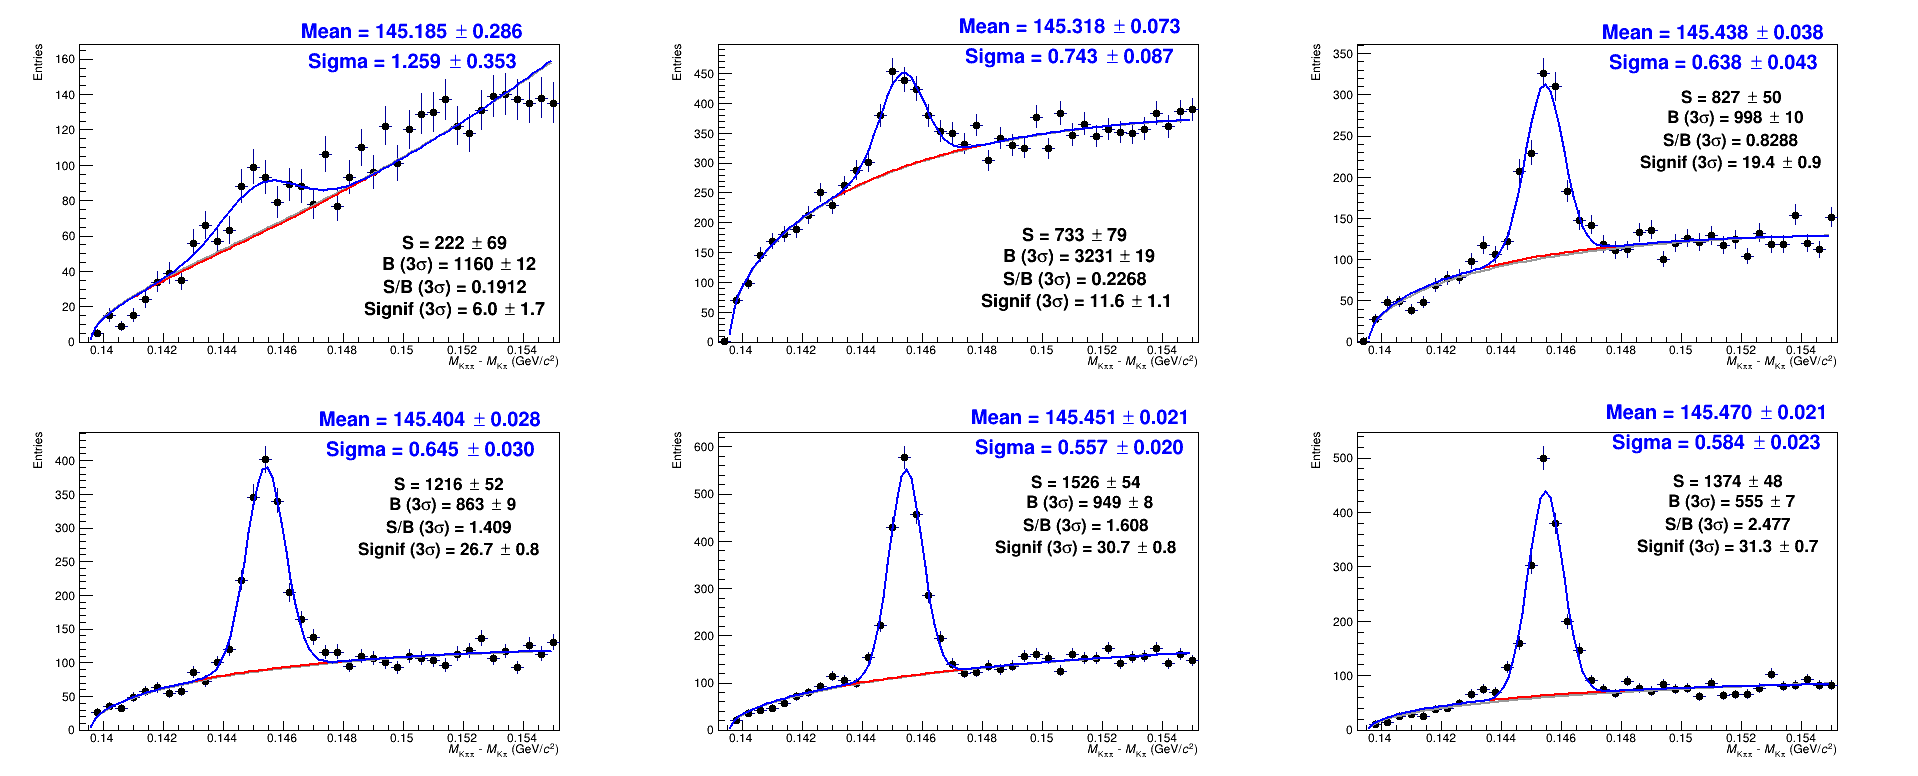
\includegraphics[width=0.7\textwidth]{figures/Dstar/pp13TeV/multi_trial/Mass_Spectra_stdBkg_1-4GeV.png} 
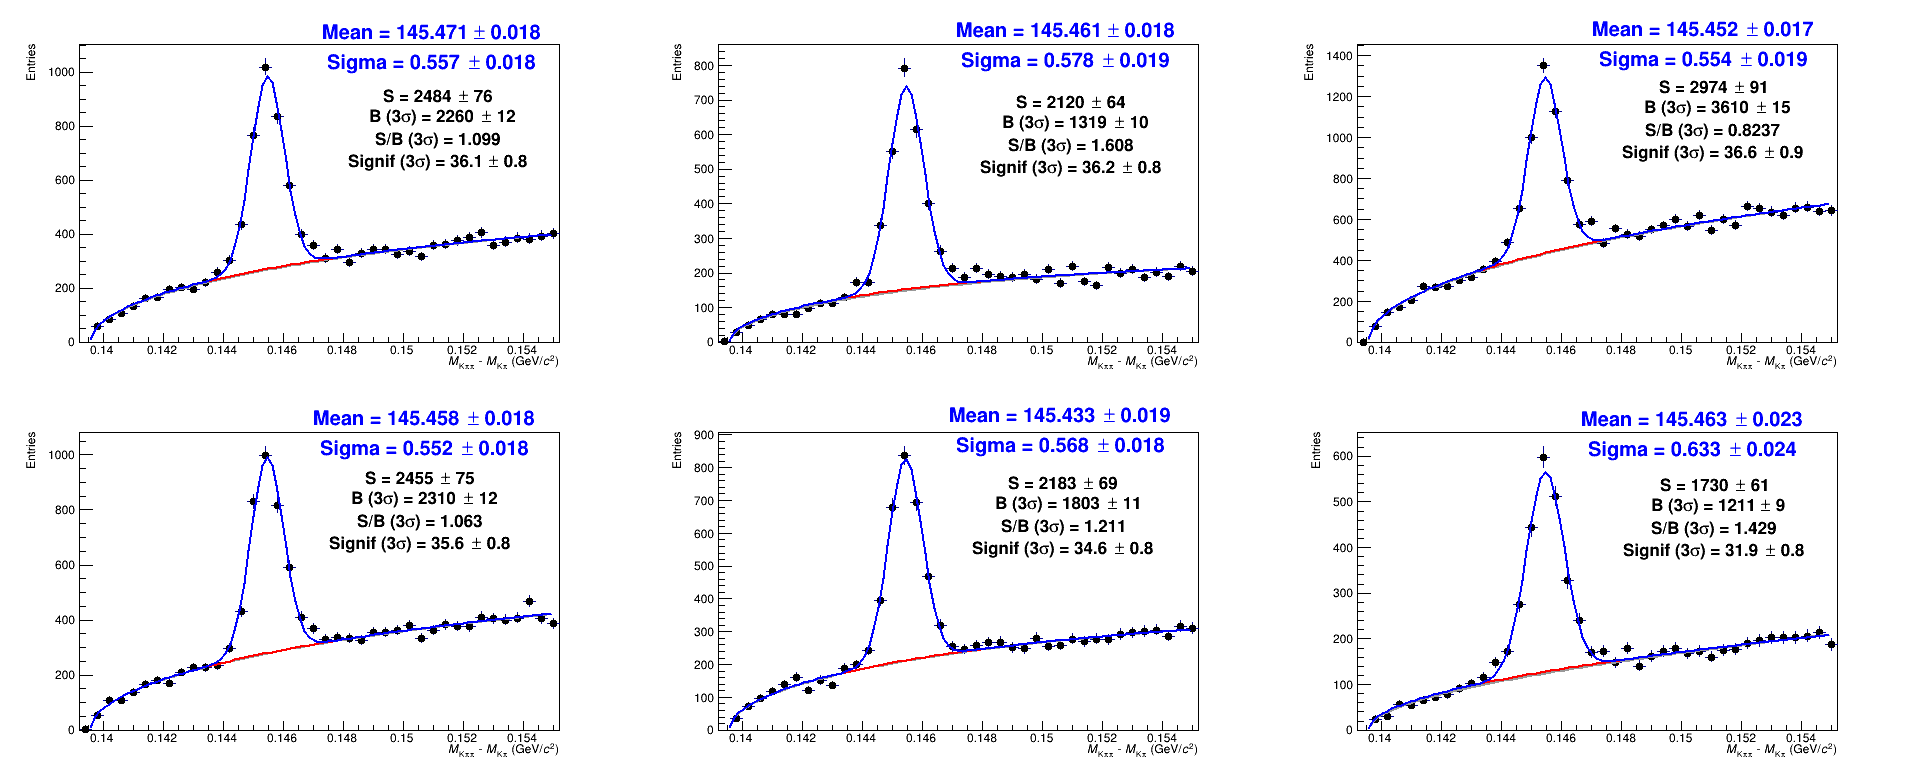
\includegraphics[width=0.7\textwidth]{figures/Dstar/pp13TeV/multi_trial/Mass_Spectra_stdBkg_4-7GeV.png}
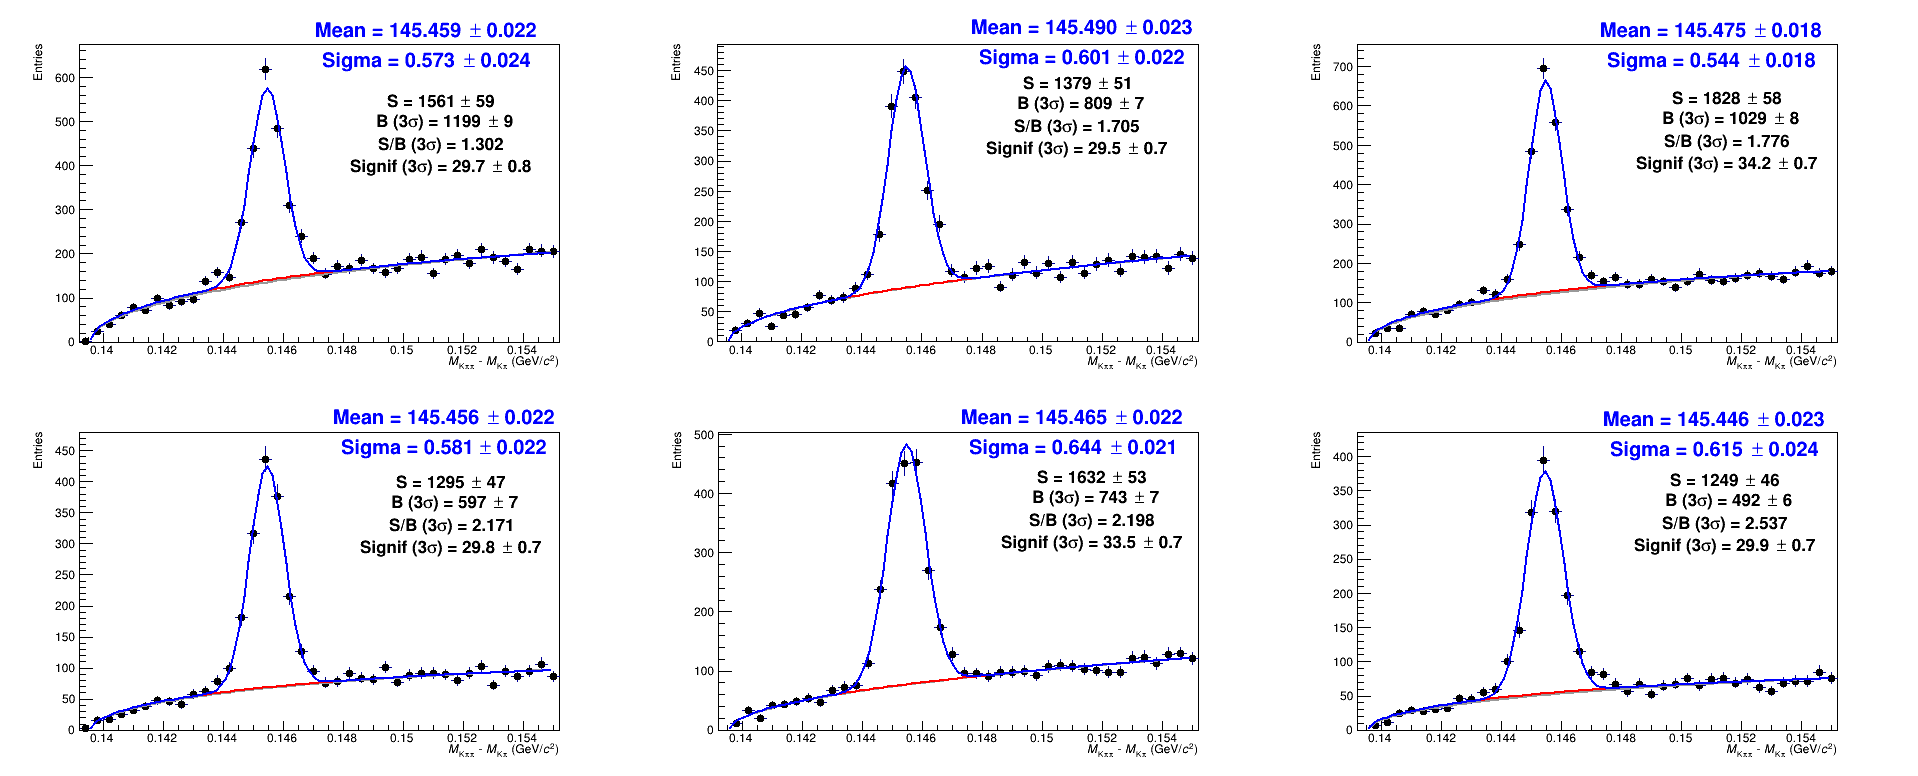
\includegraphics[width=0.7\textwidth]{figures/Dstar/pp13TeV/multi_trial/Mass_Spectra_stdBkg_7-16GeV.png}
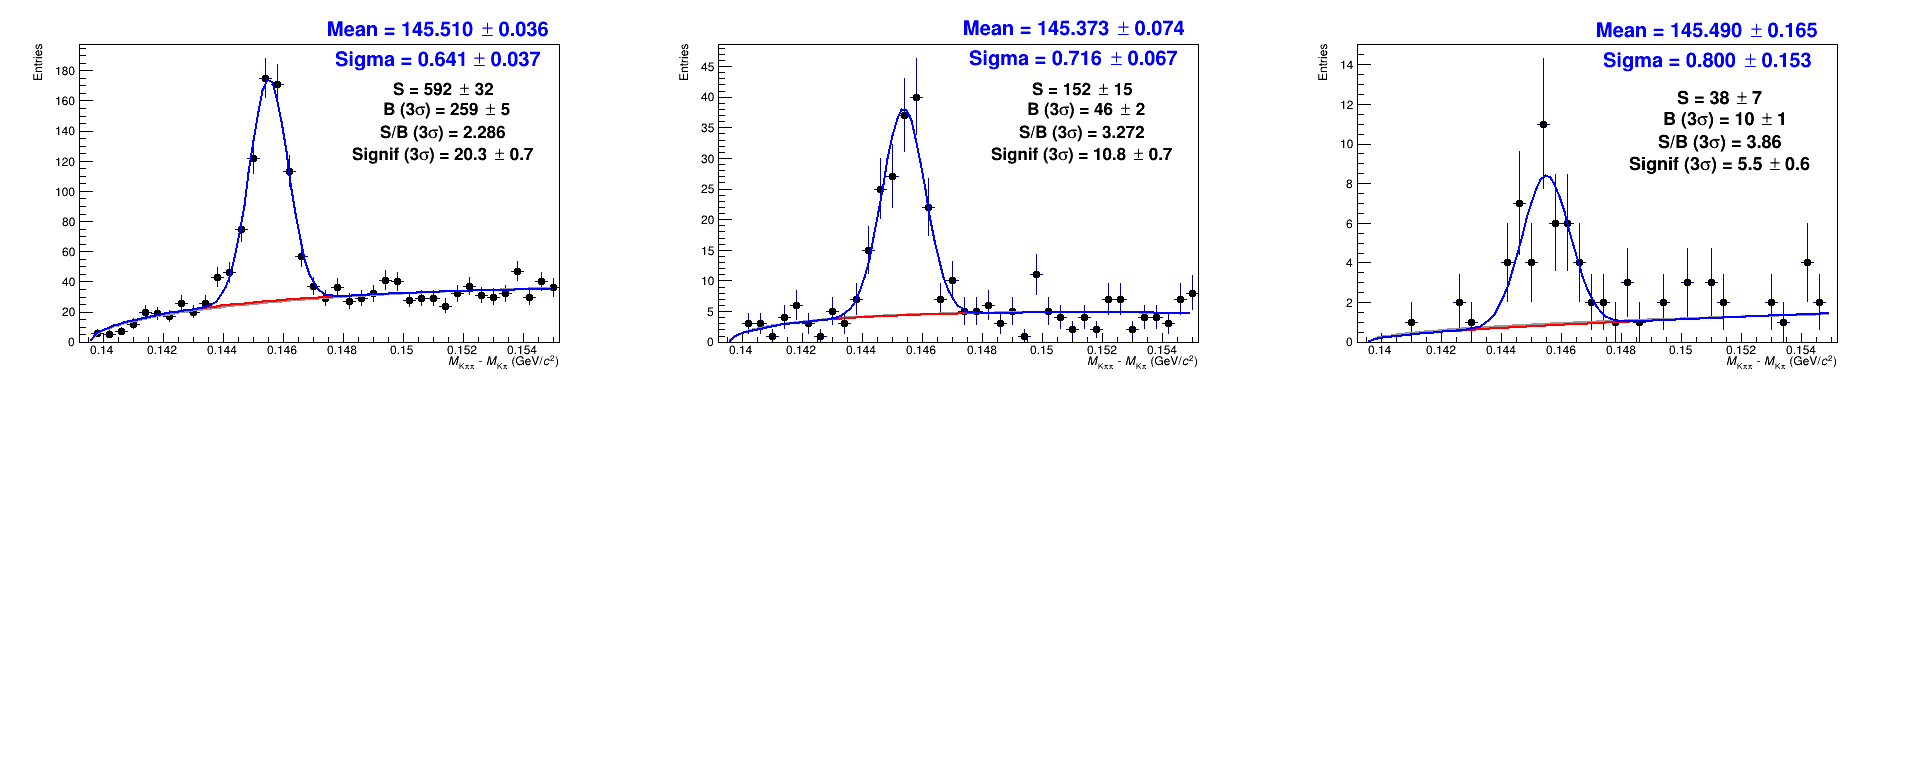
\includegraphics[width=0.7\textwidth]{figures/Dstar/pp13TeV/multi_trial/Mass_Spectra_stdBkg_16-50GeV.png} 
%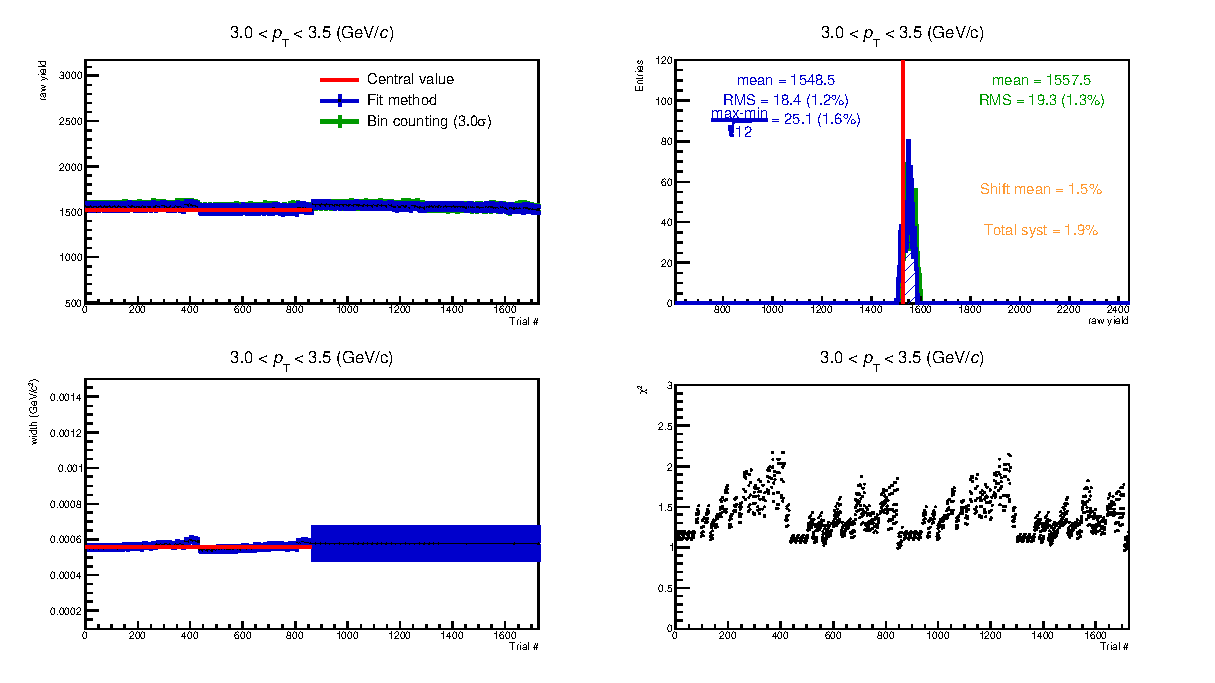
\includegraphics[width=0.8\textwidth]{figures/Dstar/pp13TeV/multi_trial/MultiFit_bkg5_3-3.eps}
%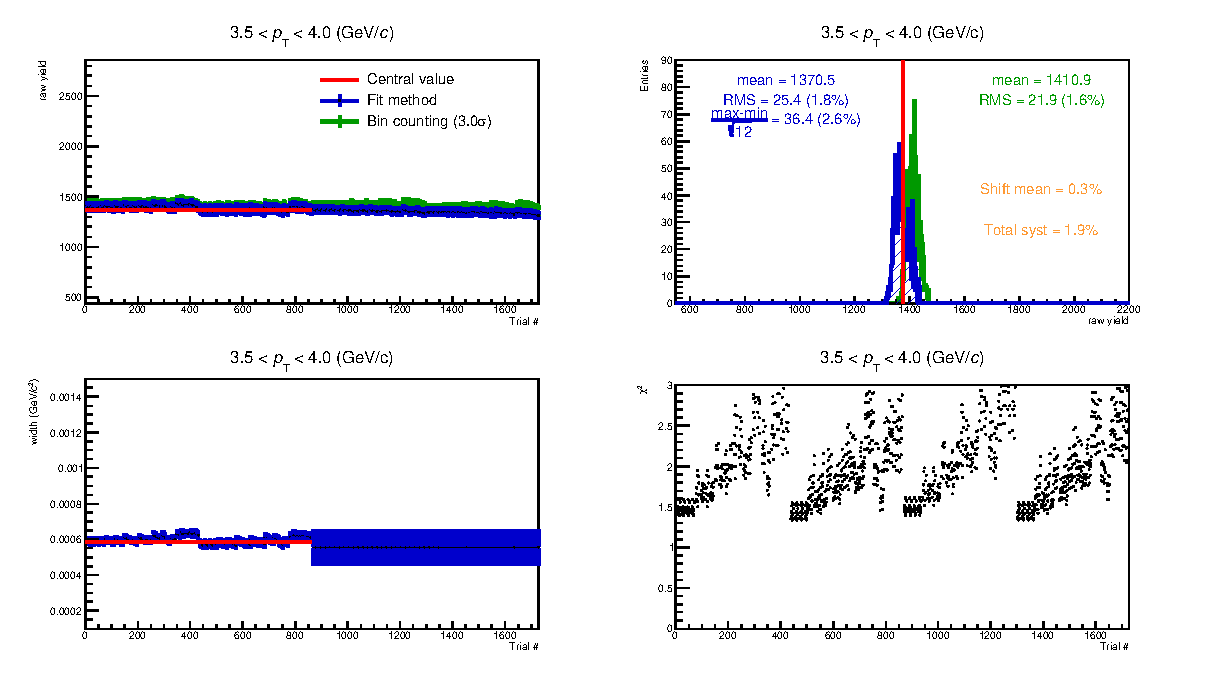
\includegraphics[width=0.65\textwidth]{figures/Dstar/pp13TeV/multi_trial/MultiFit_bkg5_3-4.eps}
%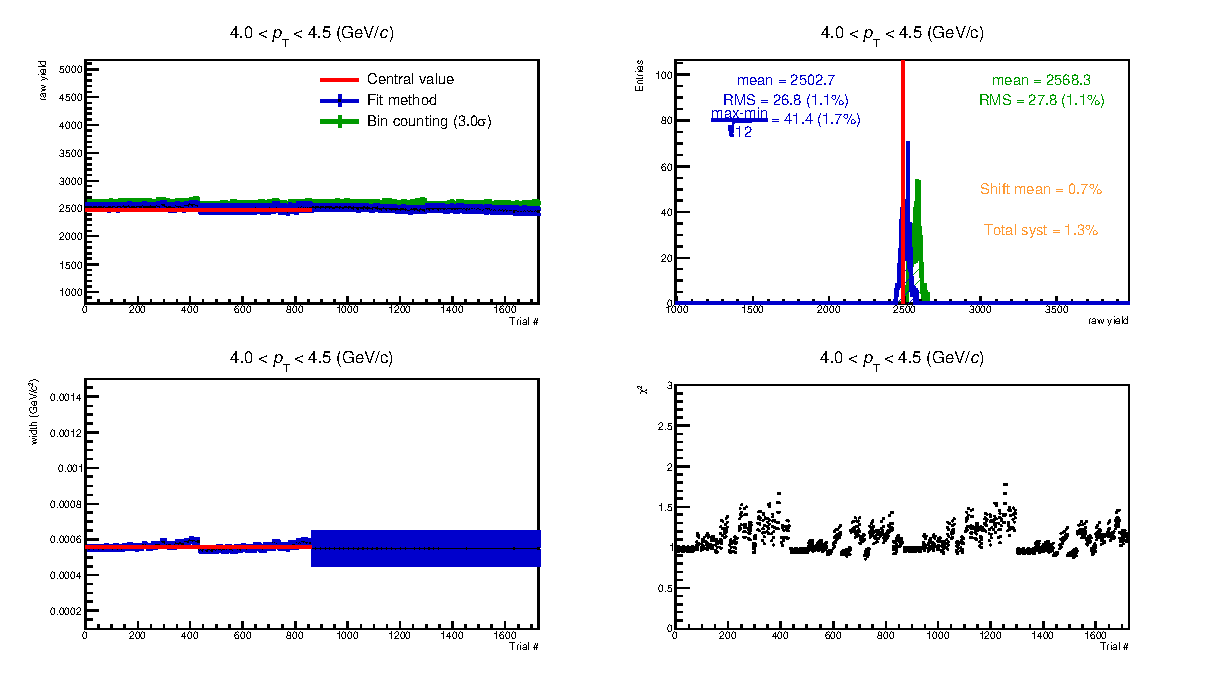
\includegraphics[width=0.65\textwidth]{figures/Dstar/pp13TeV/multi_trial/MultiFit_bkg5_4-4.eps}
\caption{\Dstar signal extraction using standard background fit function.}
\label{fig:DstarYield_stdbkg}
\end{center}
\end{figure}


\begin{figure}[!h]
\begin{center}
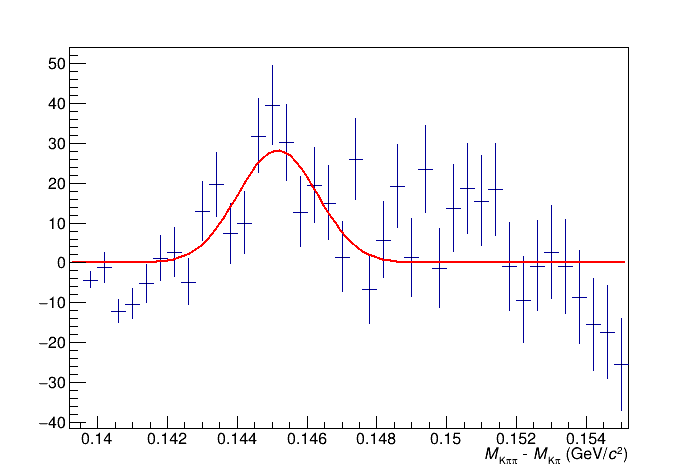
\includegraphics[width=0.3\textwidth]{figures/Dstar/pp13TeV/multi_trial/residual_plot_std_bkg_func_1-1dot5GeV.png} 
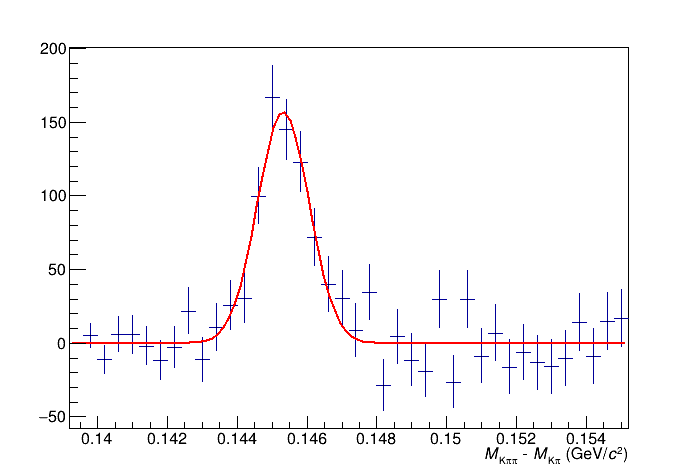
\includegraphics[width=0.3\textwidth]{figures/Dstar/pp13TeV/multi_trial/residual_plot_std_bkg_func_1dot5-2GeV.png}
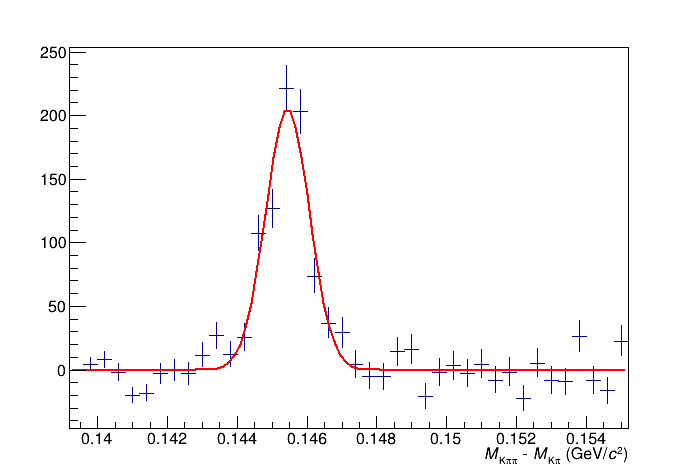
\includegraphics[width=0.3\textwidth]{figures/Dstar/pp13TeV/multi_trial/residual_plot_std_bkg_func_2-2dot5GeV.png} 

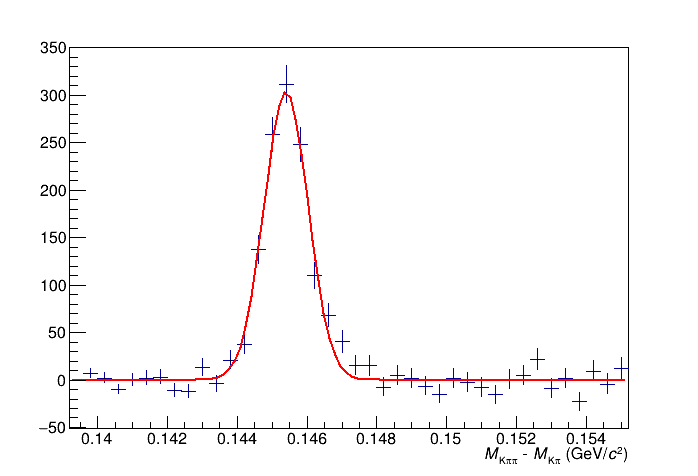
\includegraphics[width=0.3\textwidth]{figures/Dstar/pp13TeV/multi_trial/residual_plot_stdBkg_func_2dot5-3GeV.png} 
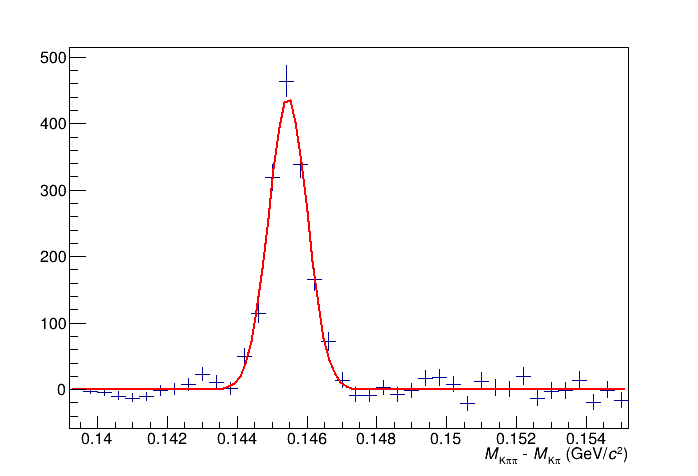
\includegraphics[width=0.3\textwidth]{figures/Dstar/pp13TeV/multi_trial/residual_plot_std_bkg_func_3-3dot5GeV.png}
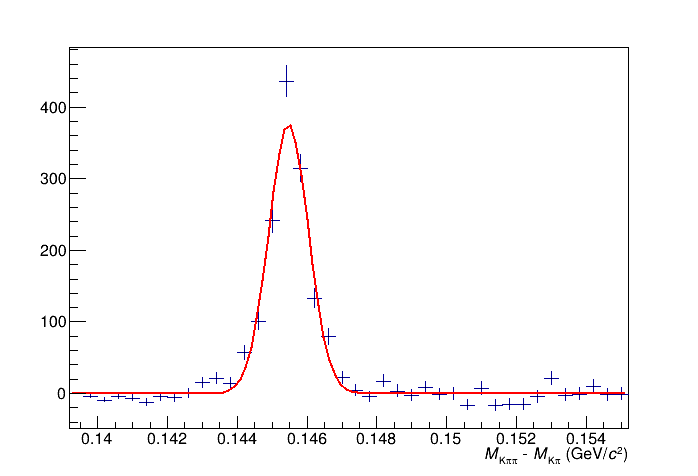
\includegraphics[width=0.3\textwidth]{figures/Dstar/pp13TeV/multi_trial/residual_plot_std_bkg_func_3dot5-4GeV.png} 

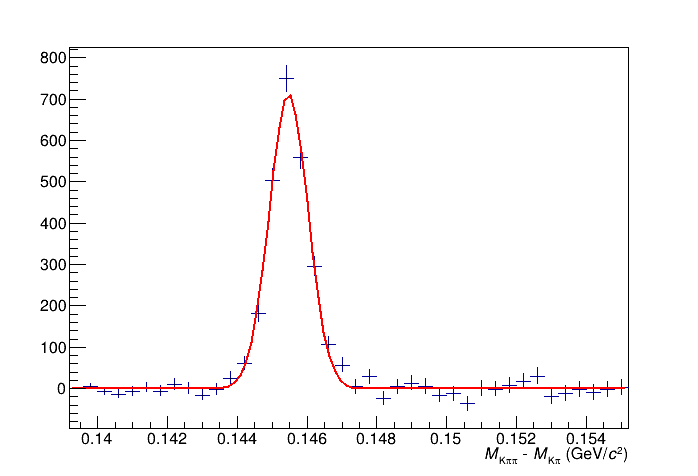
\includegraphics[width=0.3\textwidth]{figures/Dstar/pp13TeV/multi_trial/residual_plot_std_bkg_func_4-4dot5GeV.png} 
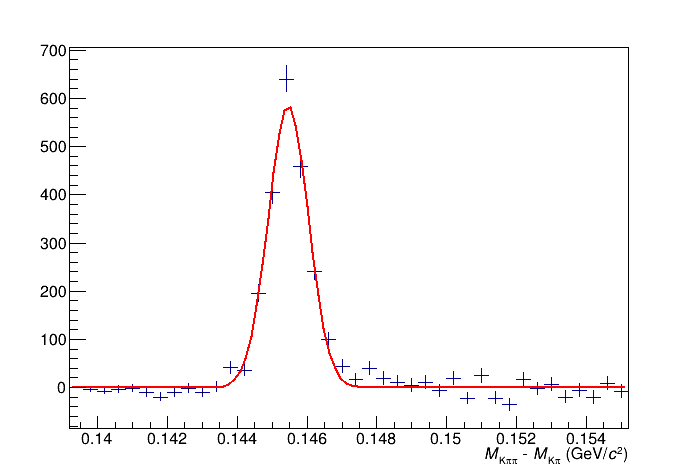
\includegraphics[width=0.3\textwidth]{figures/Dstar/pp13TeV/multi_trial/residual_plot_std_bkg_func_4dot5-5GeV.png}
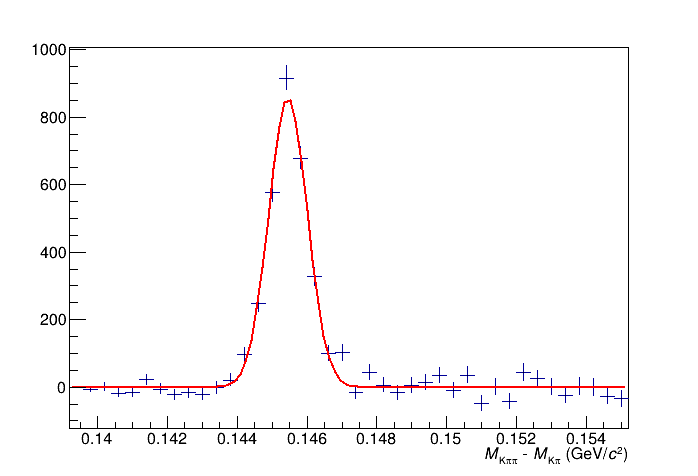
\includegraphics[width=0.3\textwidth]{figures/Dstar/pp13TeV/multi_trial/residual_plot_std_bkg_func_5-5dot5GeV.png} 

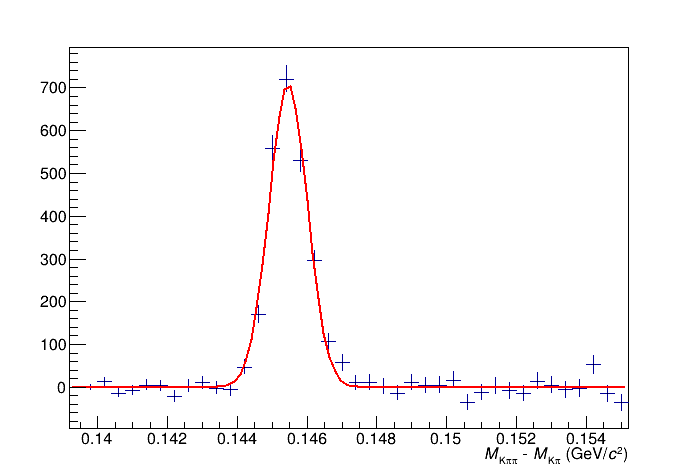
\includegraphics[width=0.3\textwidth]{figures/Dstar/pp13TeV/multi_trial/residual_plot_std_bkg_func_5dot5-6GeV.png} 
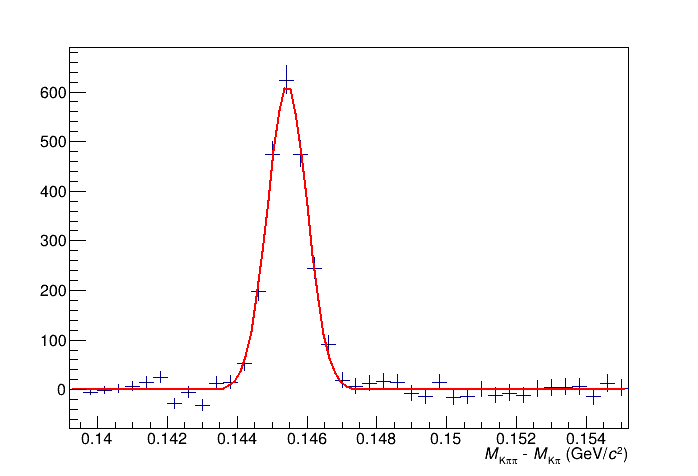
\includegraphics[width=0.3\textwidth]{figures/Dstar/pp13TeV/multi_trial/residual_plot_std_bkg_func_6-6dot5GeV.png}
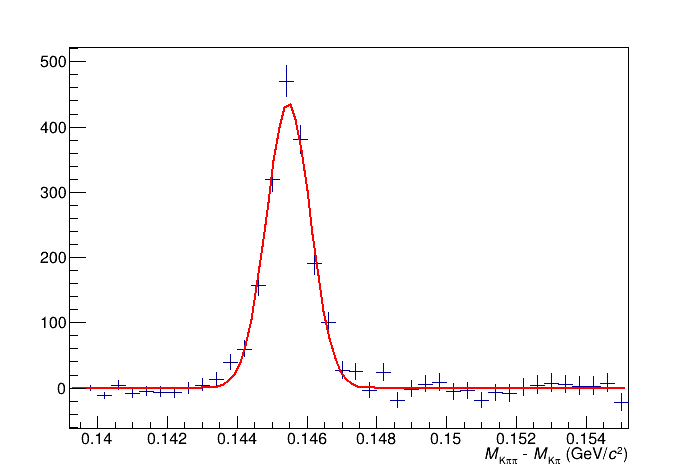
\includegraphics[width=0.3\textwidth]{figures/Dstar/pp13TeV/multi_trial/residual_plot_std_bkg_func_6dot5-7GeV.png} 

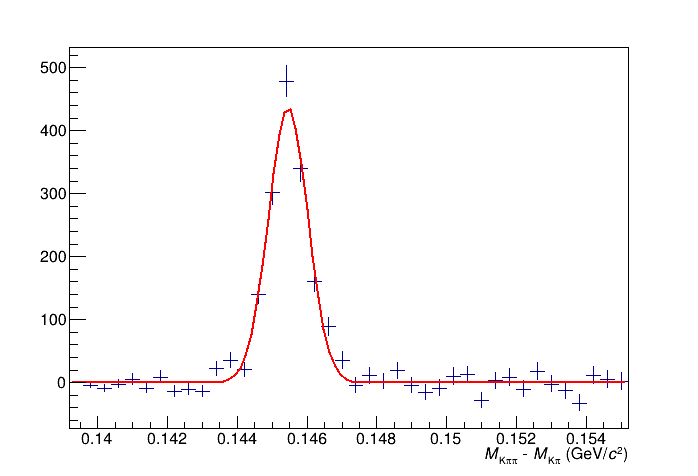
\includegraphics[width=0.3\textwidth]{figures/Dstar/pp13TeV/multi_trial/residual_plot_std_bkg_func_7-7dot5GeV.png} 
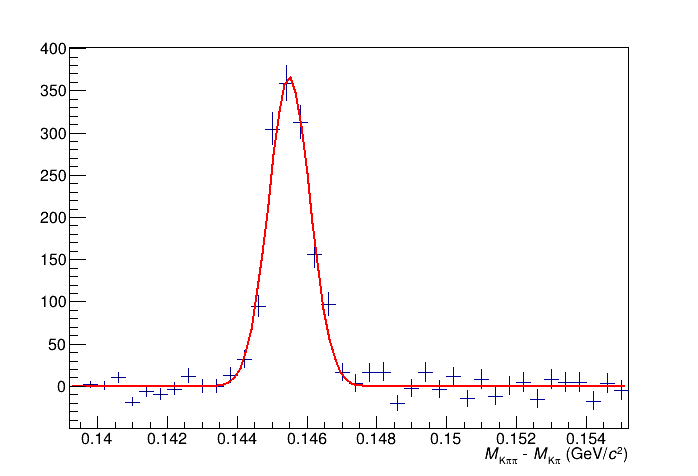
\includegraphics[width=0.3\textwidth]{figures/Dstar/pp13TeV/multi_trial/residual_plot_std_bkg_func_7dot5-8GeV.png}
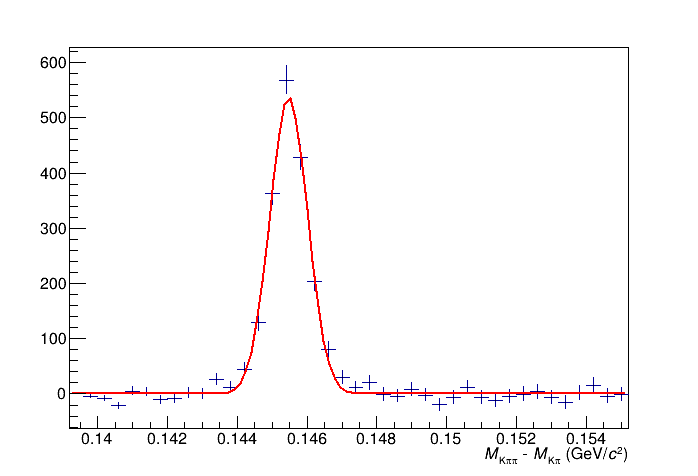
\includegraphics[width=0.3\textwidth]{figures/Dstar/pp13TeV/multi_trial/residual_plot_std_bkg_func_8-9GeV.png} 

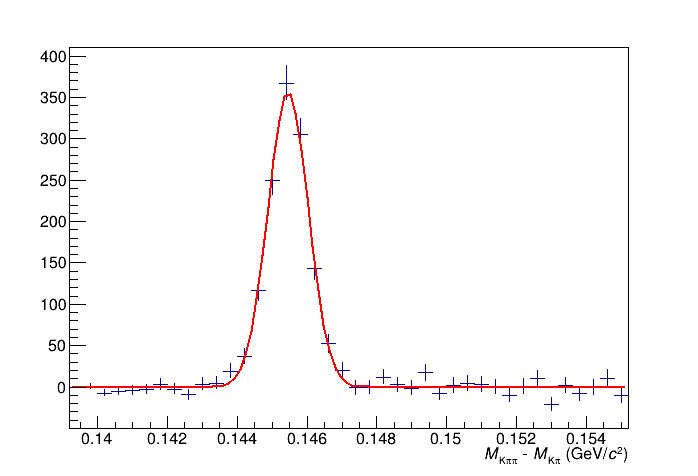
\includegraphics[width=0.3\textwidth]{figures/Dstar/pp13TeV/multi_trial/residual_plot_std_bkg_func_9-10GeV.png} 
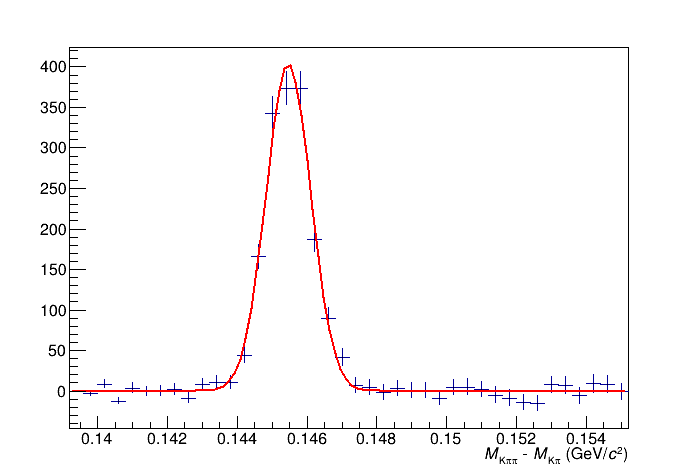
\includegraphics[width=0.3\textwidth]{figures/Dstar/pp13TeV/multi_trial/residual_plot_std_bkg_func_10-12GeV.png}
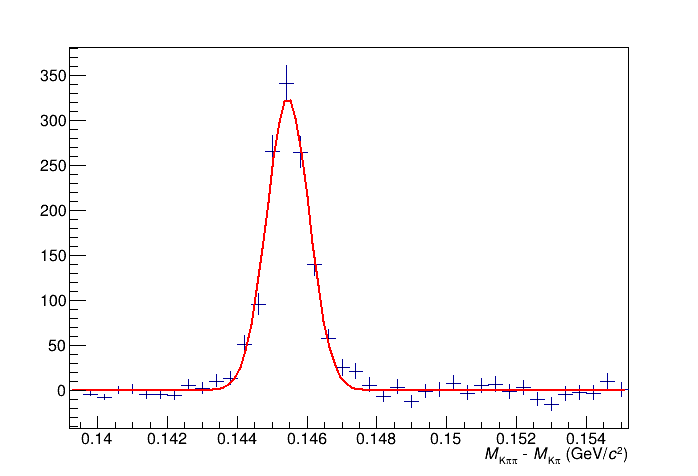
\includegraphics[width=0.3\textwidth]{figures/Dstar/pp13TeV/multi_trial/residual_plot_std_bkg_func_12-16GeV.png} 

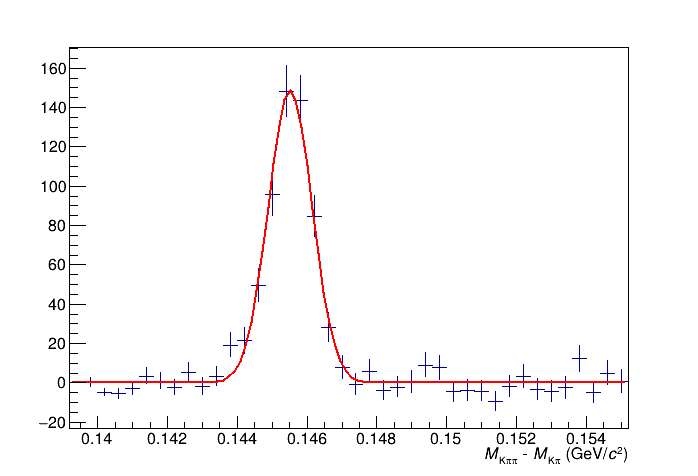
\includegraphics[width=0.3\textwidth]{figures/Dstar/pp13TeV/multi_trial/residual_plot_std_bkg_func_16-24GeV.png} 
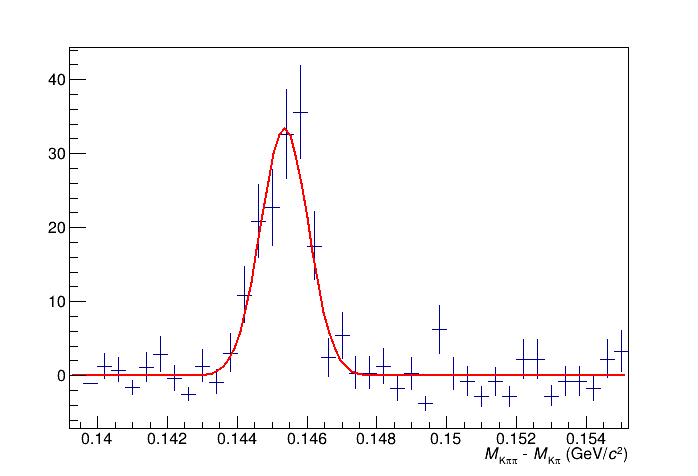
\includegraphics[width=0.3\textwidth]{figures/Dstar/pp13TeV/multi_trial/residual_plot_std_bkg_func_24-36GeV.png}
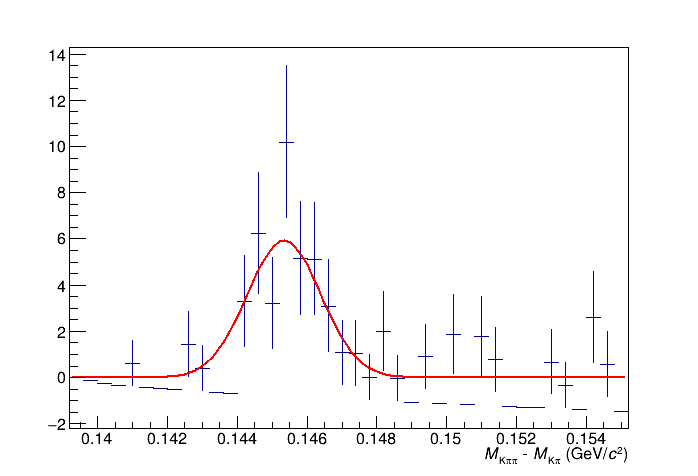
\includegraphics[width=0.3\textwidth]{figures/Dstar/pp13TeV/multi_trial/residual_plot_std_bkg_func_36-50GeV.png} 

\caption{Residual plots using standard background fit function.}
\label{fig:DstarYield_stdbkg_residual}
\end{center}
\end{figure}


\begin{figure}[!h]
\begin{center}
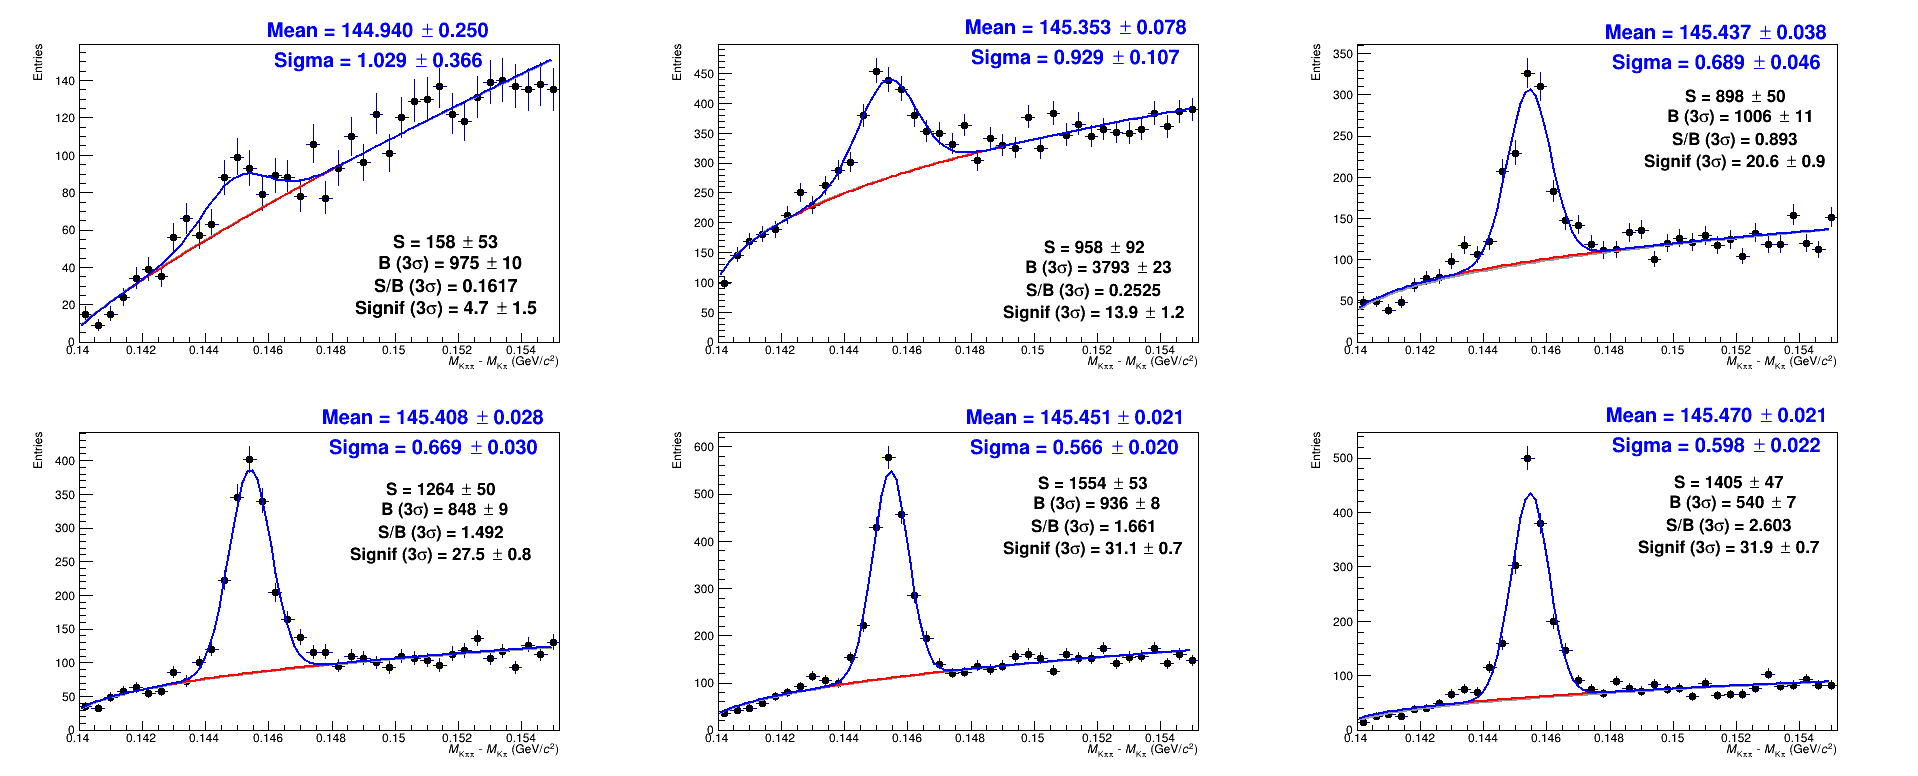
\includegraphics[width=0.7\textwidth]{figures/Dstar/pp13TeV/multi_trial/Mass_Spectra_PowerFuncBkg_1-4GeV.png} 
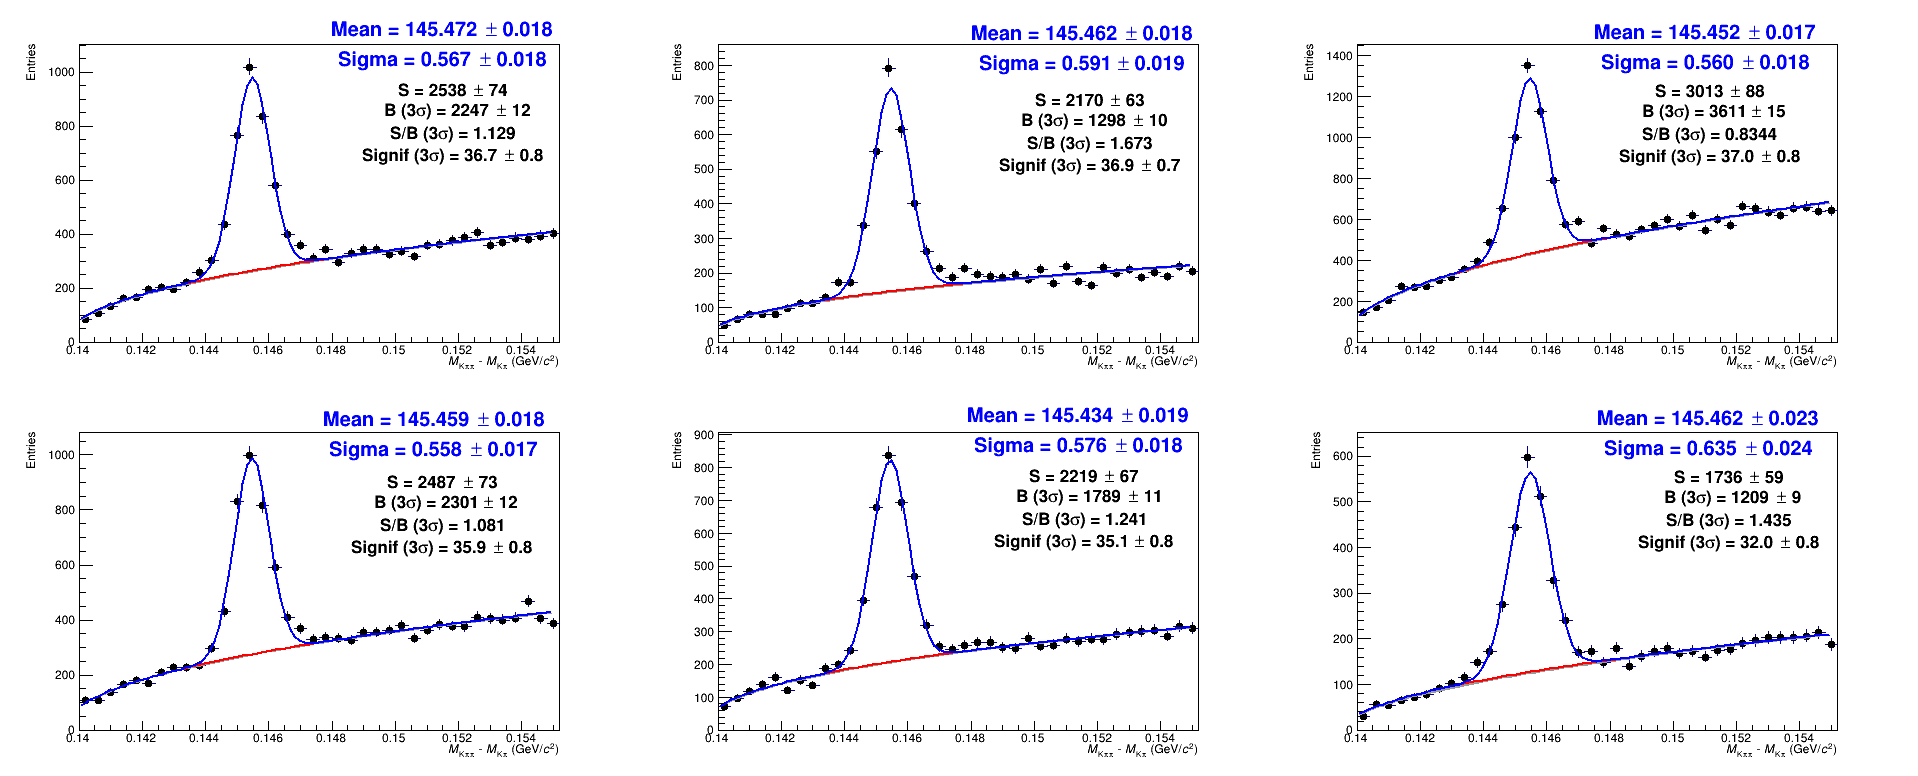
\includegraphics[width=0.7\textwidth]{figures/Dstar/pp13TeV/multi_trial/Mass_Spectra_PowerFuncBkg_4-7GeV.png}
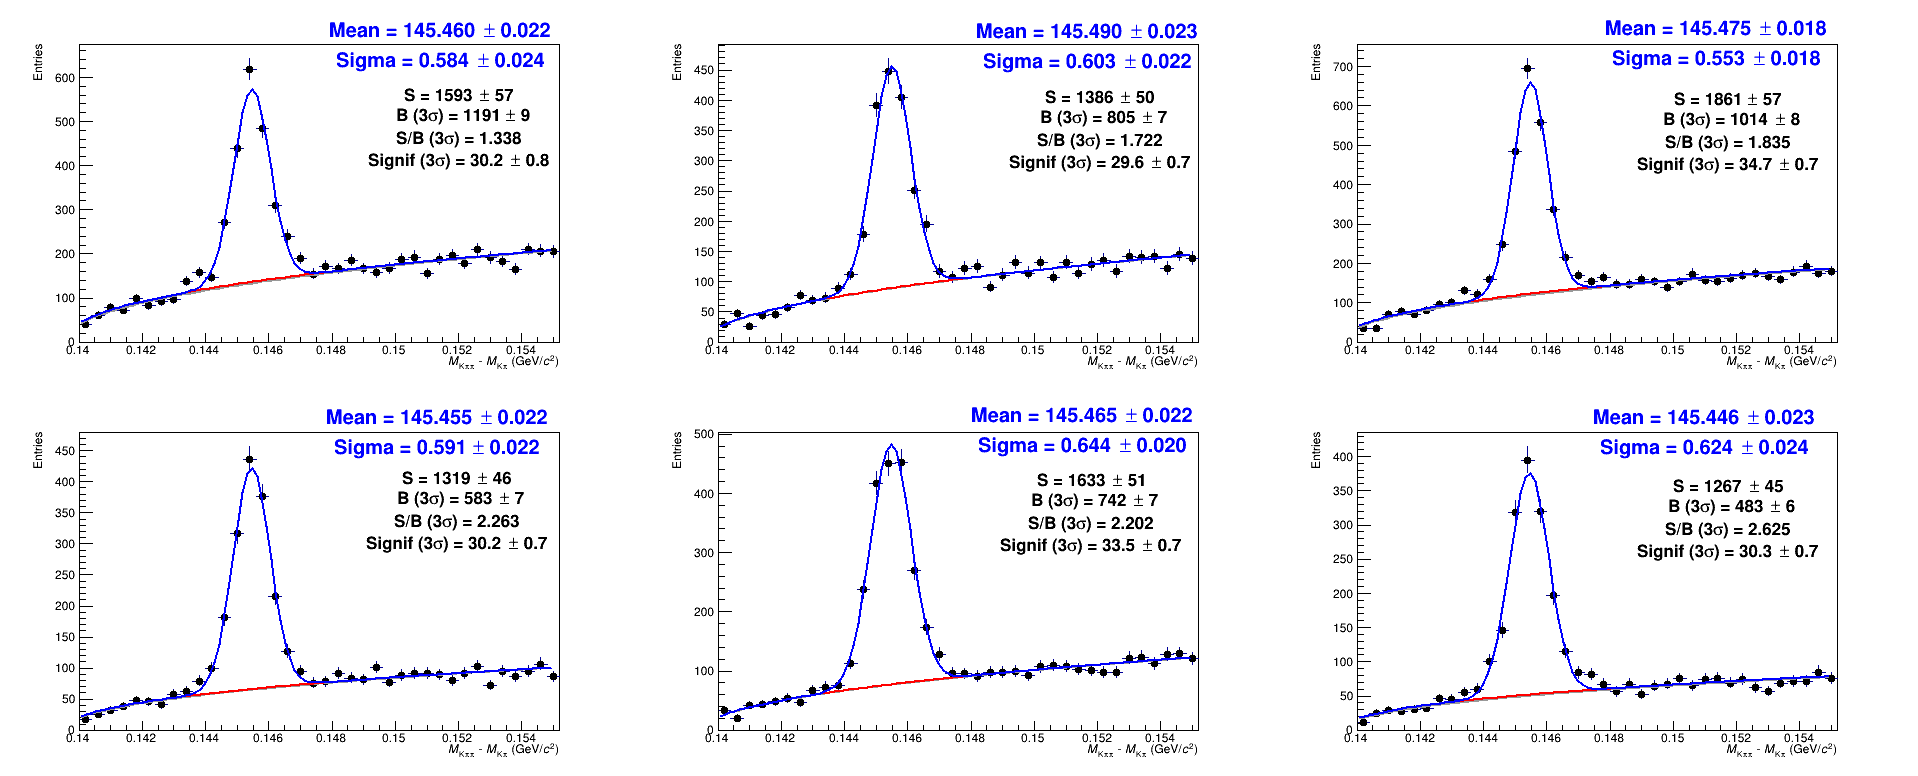
\includegraphics[width=0.7\textwidth]{figures/Dstar/pp13TeV/multi_trial/Mass_Spectra_PowerFuncBkg_7-16GeV.png}
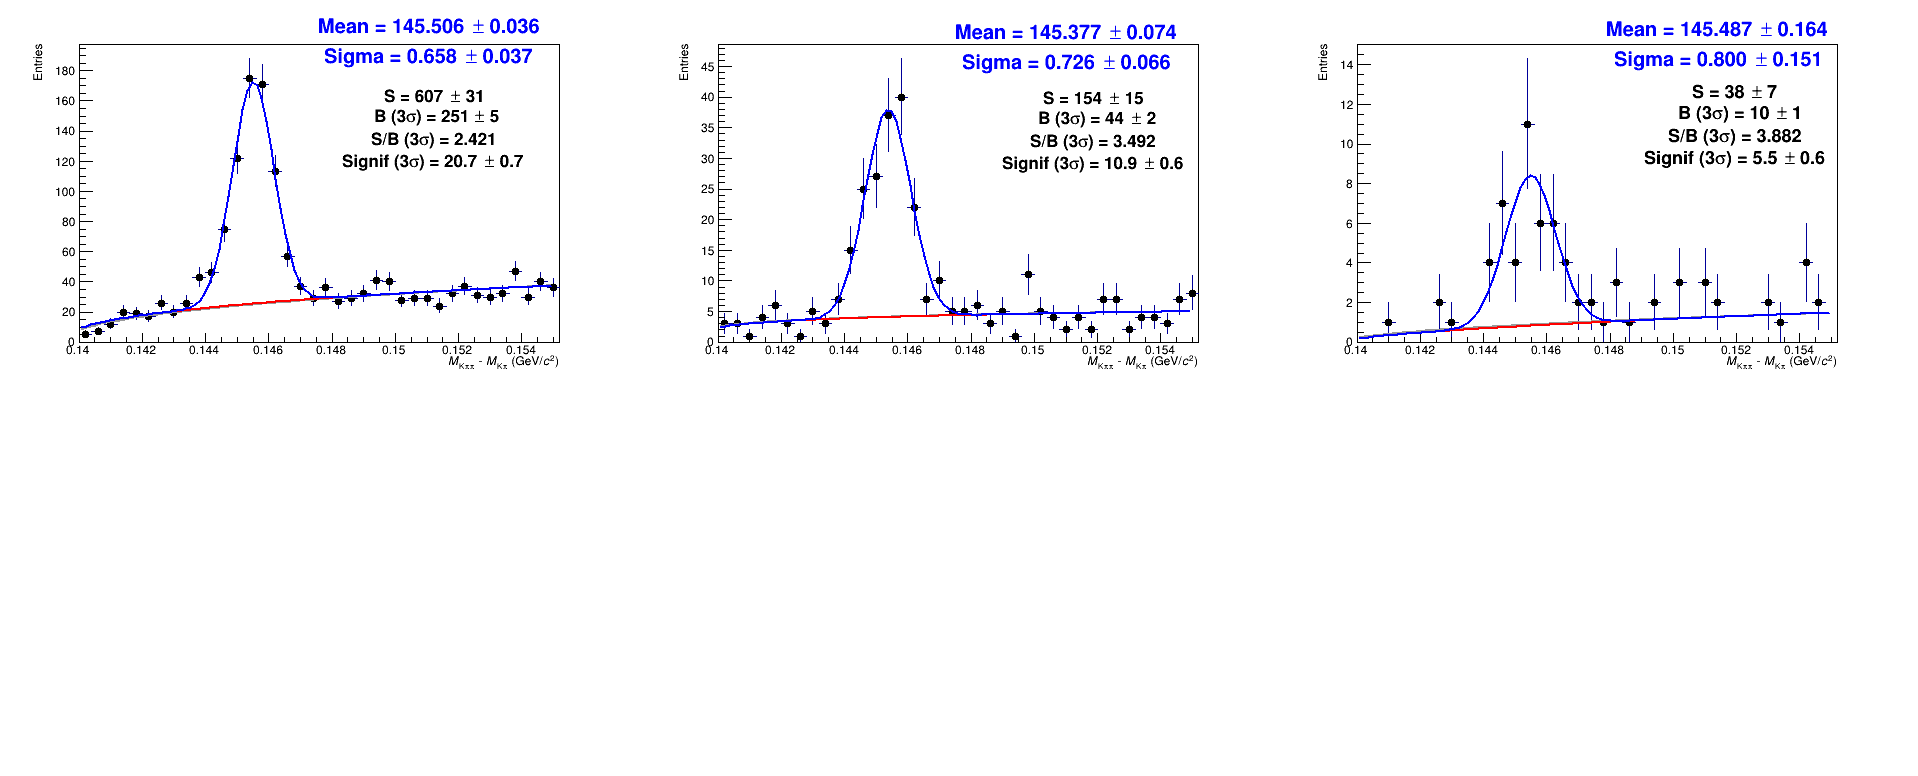
\includegraphics[width=0.7\textwidth]{figures/Dstar/pp13TeV/multi_trial/Mass_Spectra_PowerFuncBkg_16-50GeV.png} 
%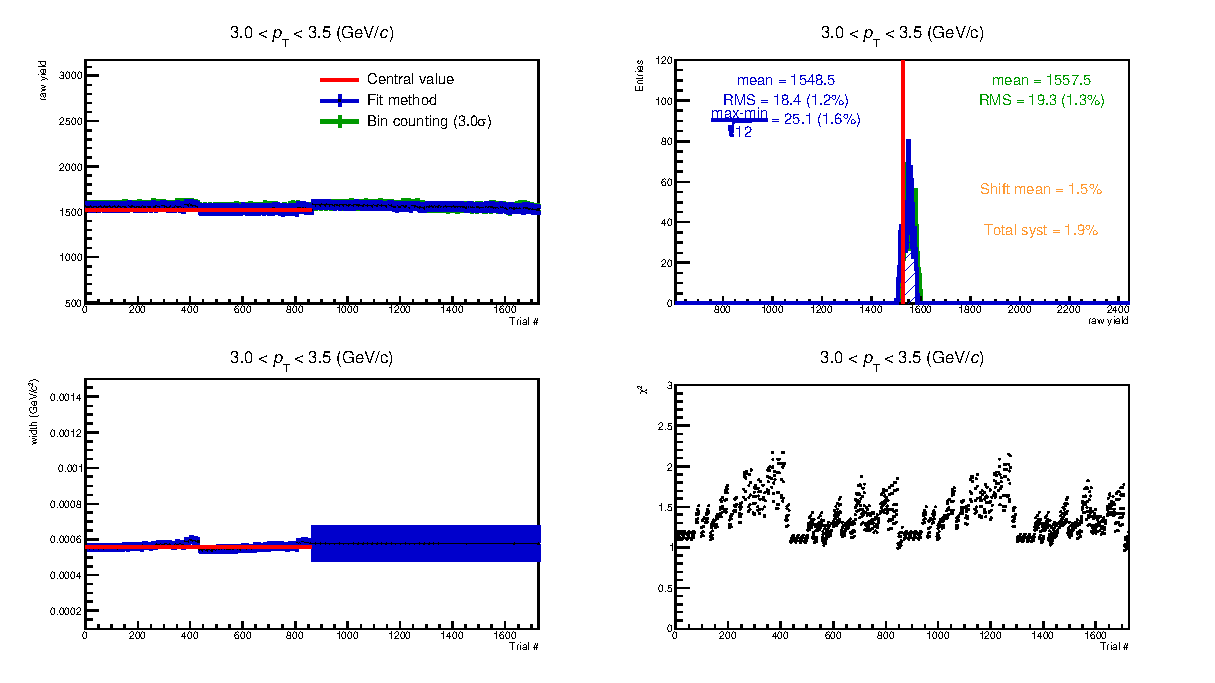
\includegraphics[width=0.8\textwidth]{figures/Dstar/pp13TeV/multi_trial/MultiFit_bkg5_3-3.eps}
%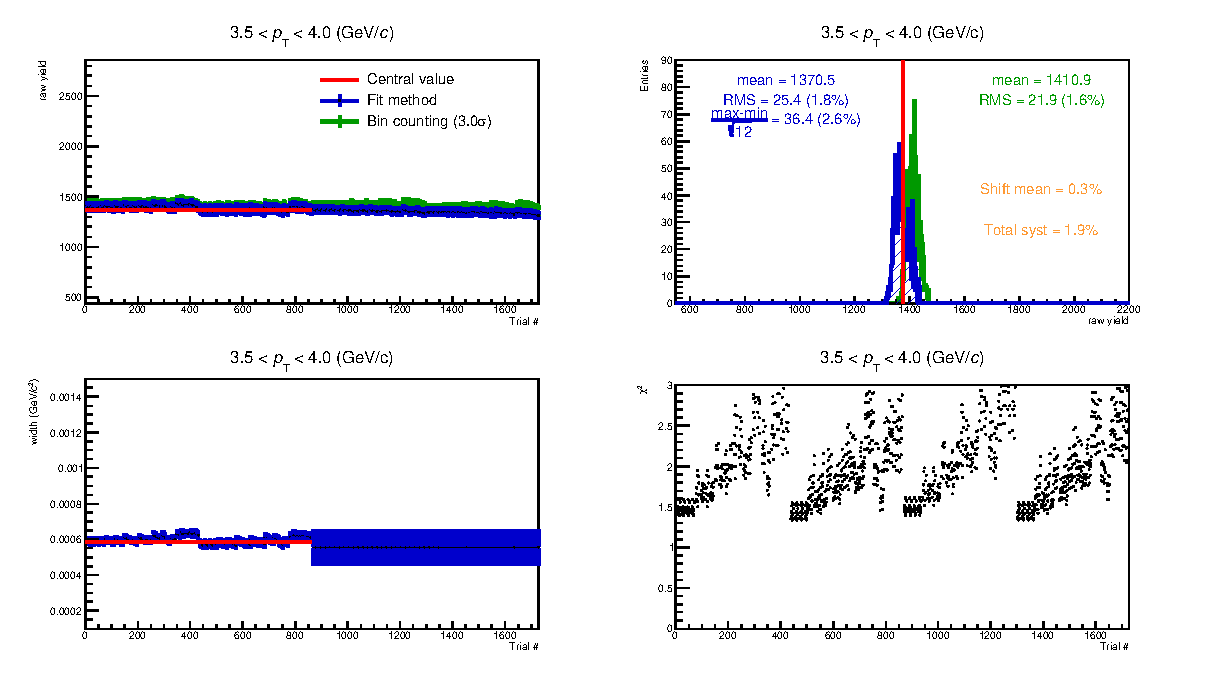
\includegraphics[width=0.65\textwidth]{figures/Dstar/pp13TeV/multi_trial/MultiFit_bkg5_3-4.eps}
%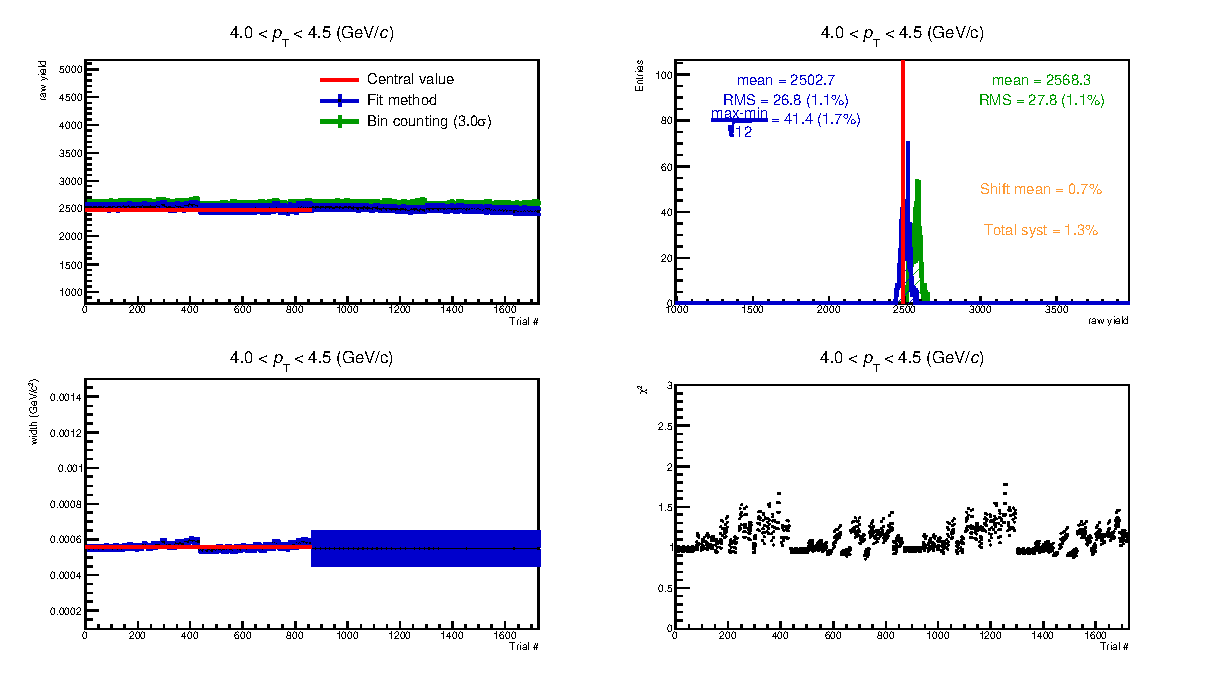
\includegraphics[width=0.65\textwidth]{figures/Dstar/pp13TeV/multi_trial/MultiFit_bkg5_4-4.eps}
\caption{\Dstar signal extraction using Power fit function for background.}
\label{fig:DstarYield_Powerbkg}
\end{center}
\end{figure}

\begin{figure}[!h]
\begin{center}
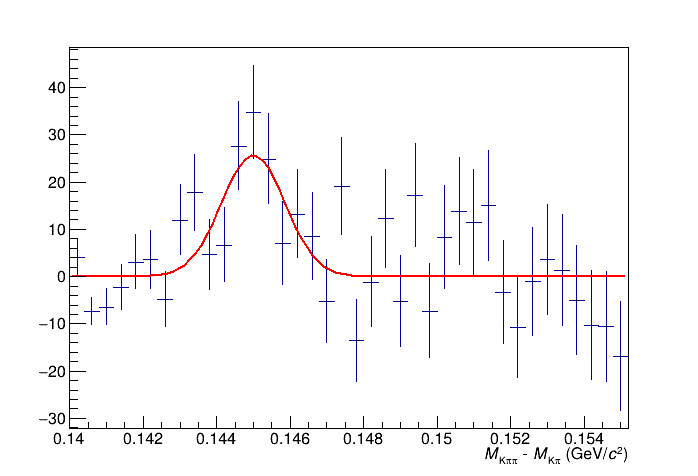
\includegraphics[width=0.3\textwidth]{figures/Dstar/pp13TeV/multi_trial/residual_plot_Pow_bkg_func_1-1dot5GeV.png} 
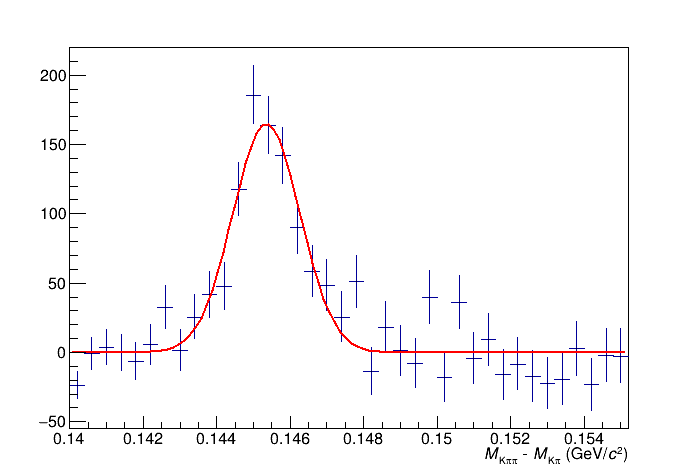
\includegraphics[width=0.3\textwidth]{figures/Dstar/pp13TeV/multi_trial/residual_plot_Pow_bkg_func_1dot5-2GeV.png}
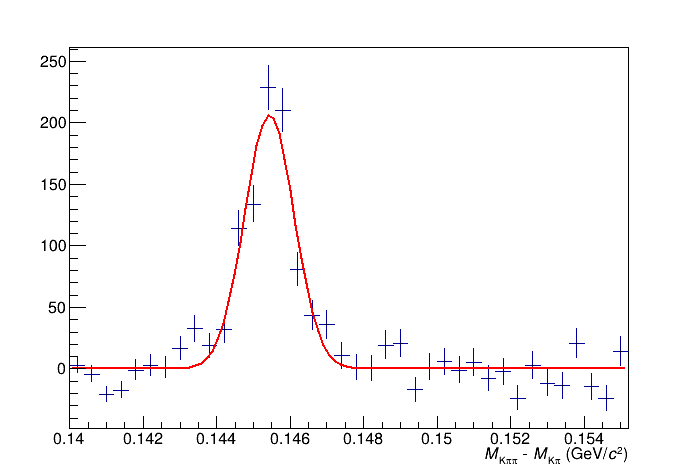
\includegraphics[width=0.3\textwidth]{figures/Dstar/pp13TeV/multi_trial/residual_plot_Pow_bkg_func_2-2dot5GeV.png} 

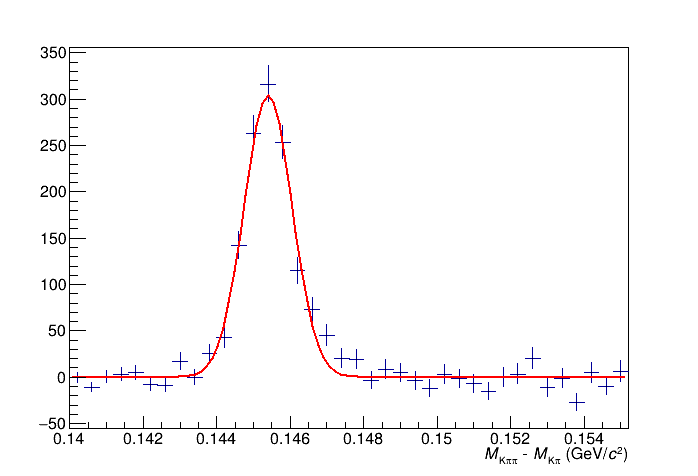
\includegraphics[width=0.3\textwidth]{figures/Dstar/pp13TeV/multi_trial/residual_plot_Pow_bkg_func_2dot5-3GeV.png} 
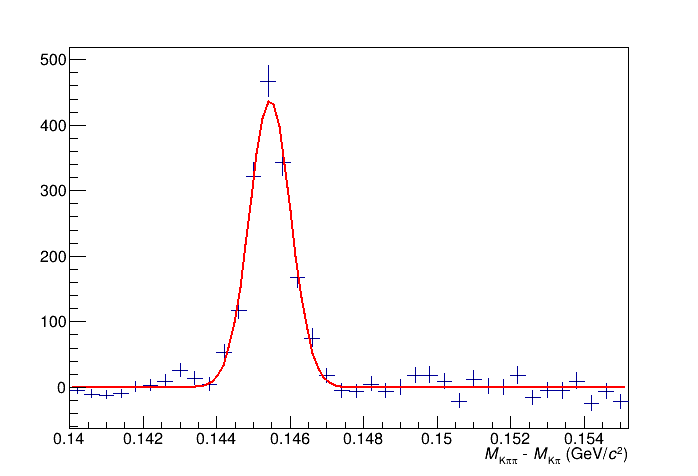
\includegraphics[width=0.3\textwidth]{figures/Dstar/pp13TeV/multi_trial/residual_plot_Pow_bkg_func_3-3dot5GeV.png}
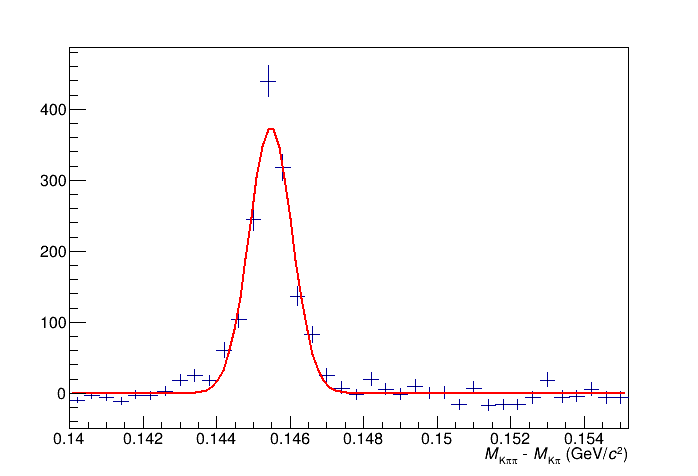
\includegraphics[width=0.3\textwidth]{figures/Dstar/pp13TeV/multi_trial/residual_plot_Pow_bkg_func_3dot5-4GeV.png} 

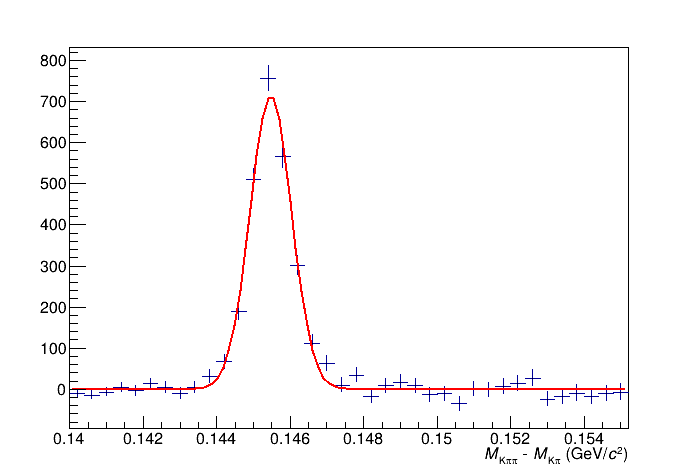
\includegraphics[width=0.3\textwidth]{figures/Dstar/pp13TeV/multi_trial/residual_plot_Pow_bkg_func_4-4dot5GeV.png} 
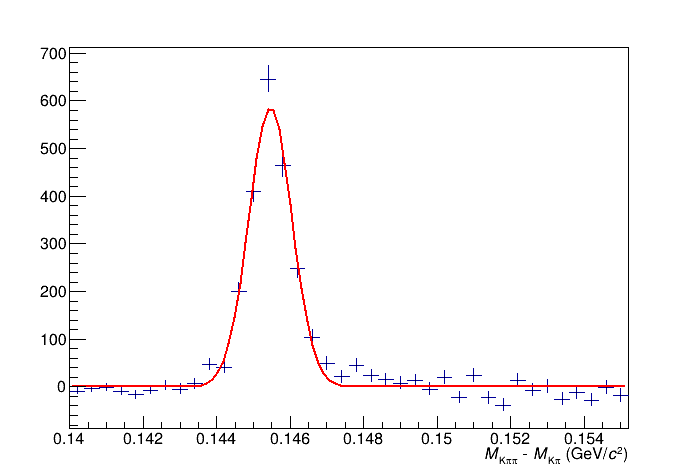
\includegraphics[width=0.3\textwidth]{figures/Dstar/pp13TeV/multi_trial/residual_plot_Pow_bkg_func_4dot5-5GeV.png}
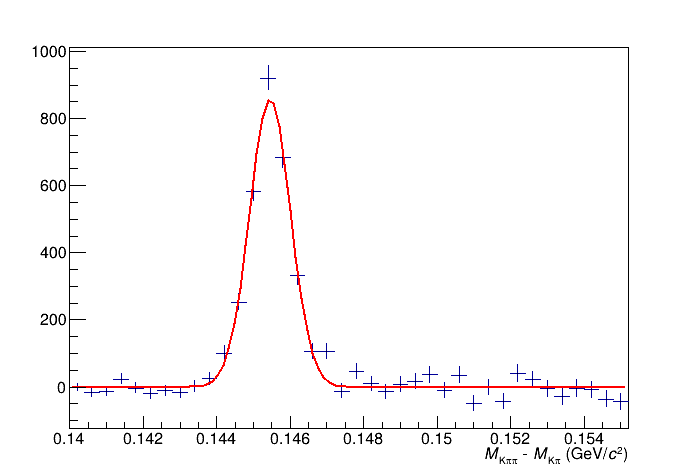
\includegraphics[width=0.3\textwidth]{figures/Dstar/pp13TeV/multi_trial/residual_plot_Pow_bkg_func_5-5dot5GeV.png} 

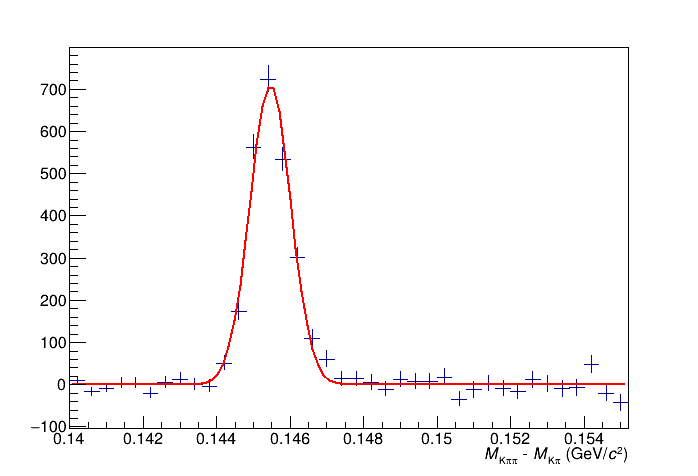
\includegraphics[width=0.3\textwidth]{figures/Dstar/pp13TeV/multi_trial/residual_plot_Pow_bkg_func_5dot5-6GeV.png} 
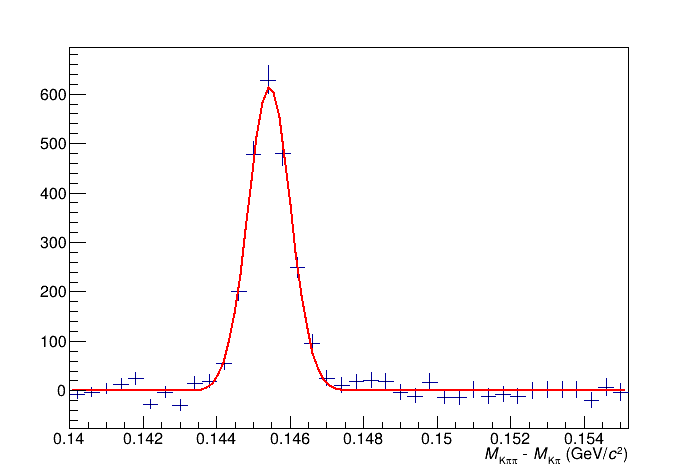
\includegraphics[width=0.3\textwidth]{figures/Dstar/pp13TeV/multi_trial/residual_plot_Pow_bkg_func_6-6dot5GeV.png}
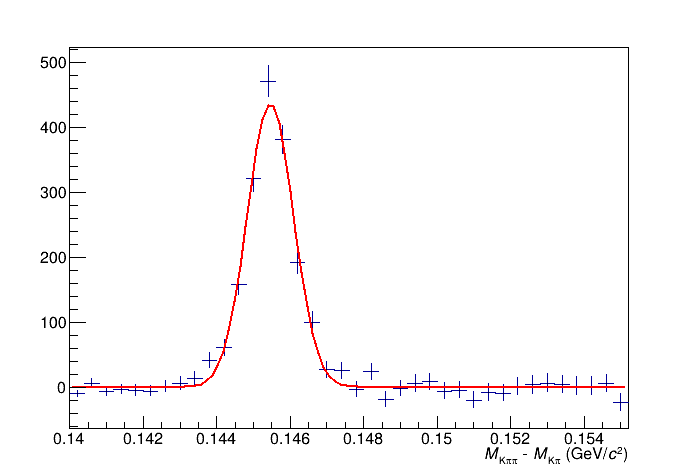
\includegraphics[width=0.3\textwidth]{figures/Dstar/pp13TeV/multi_trial/residual_plot_Pow_bkg_func_6dot5-7GeV.png} 

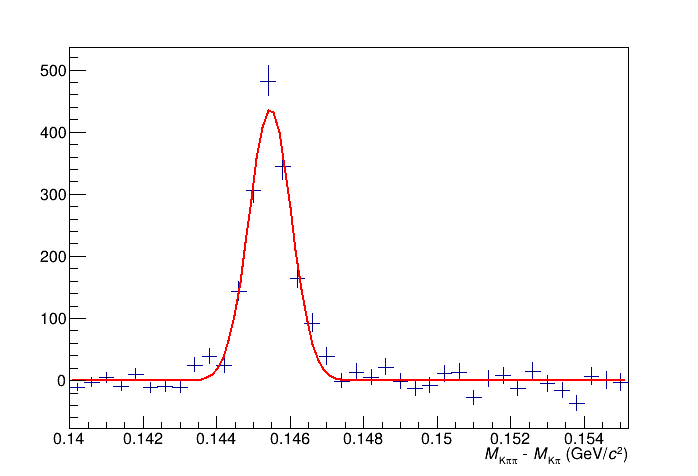
\includegraphics[width=0.3\textwidth]{figures/Dstar/pp13TeV/multi_trial/residual_plot_Pow_bkg_func_7-7dot5GeV.png} 
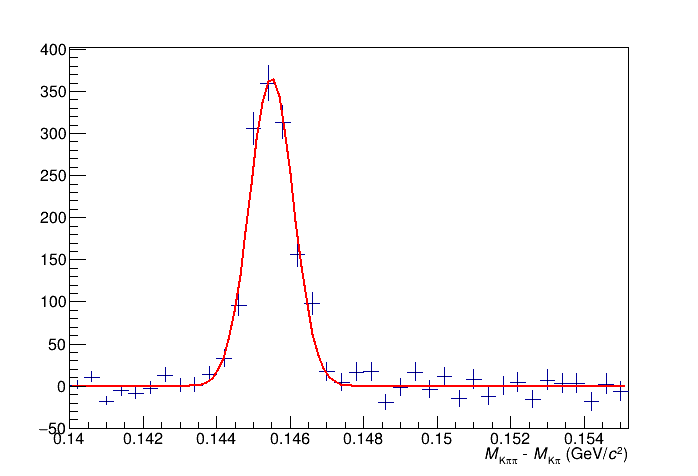
\includegraphics[width=0.3\textwidth]{figures/Dstar/pp13TeV/multi_trial/residual_plot_Pow_bkg_func_7dot5-8GeV.png}
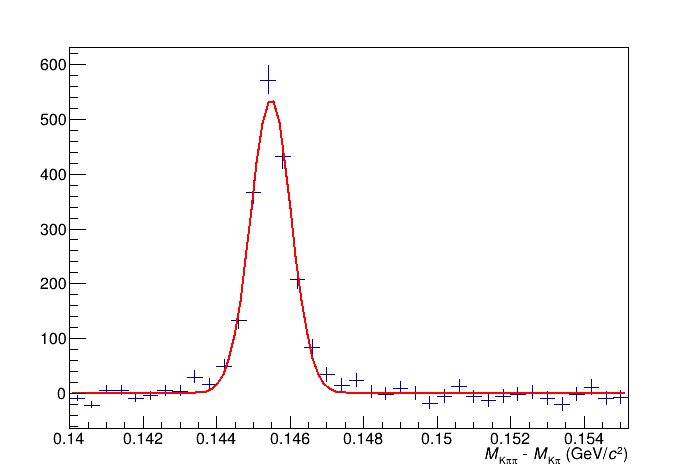
\includegraphics[width=0.3\textwidth]{figures/Dstar/pp13TeV/multi_trial/residual_plot_Pow_bkg_func_8-9GeV.png} 

\includegraphics[width=0.3\textwidth]{figures/Dstar/pp13TeV/multi_trial/residual_plot_Pow_bkg_func_9-10GeV.png} 
\includegraphics[width=0.3\textwidth]{figures/Dstar/pp13TeV/multi_trial/residual_plot_Pow_bkg_func_10-12GeV.png}
\includegraphics[width=0.3\textwidth]{figures/Dstar/pp13TeV/multi_trial/residual_plot_Pow_bkg_func_12-16GeV.png} 

\includegraphics[width=0.3\textwidth]{figures/Dstar/pp13TeV/multi_trial/residual_plot_Pow_bkg_func_16-24GeV.png} 
\includegraphics[width=0.3\textwidth]{figures/Dstar/pp13TeV/multi_trial/residual_plot_Pow_bkg_func_24-36GeV.png}
\includegraphics[width=0.3\textwidth]{figures/Dstar/pp13TeV/multi_trial/residual_plot_Pow_bkg_func_36-50GeV.png} 

\caption{Residual plots using Power fit function for background.}
\label{fig:DstarYield_residual_power}
\end{center}
\end{figure}






%======= Dstar 0-10======= multi-trial ===========

\begin{figure}[!h]
\begin{center}
\includegraphics[width=0.68\textwidth]{figures/Dstar/pp13TeV/multi_trial/MultiFit_bkg4-Okt24_1-1.eps} 
\includegraphics[width=0.68\textwidth]{figures/Dstar/pp13TeV/multi_trial/MultiFit_bkg5-Okt24_1-2.eps}
\includegraphics[width=0.68\textwidth]{figures/Dstar/pp13TeV/multi_trial/MultiFit_bkg4-24Okt_2-2.eps}
\includegraphics[width=0.68\textwidth]{figures/Dstar/pp13TeV/multi_trial/MultiFit_bkg5_2-3.eps} 
%\includegraphics[width=0.8\textwidth]{figures/Dstar/pp13TeV/multi_trial/MultiFit_bkg5_3-3.eps}
%\includegraphics[width=0.65\textwidth]{figures/Dstar/pp13TeV/multi_trial/MultiFit_bkg5_3-4.eps}
%\includegraphics[width=0.65\textwidth]{figures/Dstar/pp13TeV/multi_trial/MultiFit_bkg5_4-4.eps}
\caption{Output of the multi-trial study for \Dstar mesons for $1<$ \pt$<3$ $\GeV/c$. For each \pt bin: the top panel shows the raw yield as a function of trials and raw yield distributions, the bottom panel shows the width and $\chi^2$ as a function of trials.}
\label{fig:DstarYieldSyst010_1}
\end{center}
\end{figure}


\begin{figure}[!h]
\begin{center}
\includegraphics[width=0.68\textwidth]{figures/Dstar/pp13TeV/multi_trial/MultiFit_bkg5_3-3.eps}
\includegraphics[width=0.68\textwidth]{figures/Dstar/pp13TeV/multi_trial/MultiFit_bkg5_3-4.eps}
\includegraphics[width=0.68\textwidth]{figures/Dstar/pp13TeV/multi_trial/MultiFit_bkg5_4-4.eps}
\includegraphics[width=0.68\textwidth]{figures/Dstar/pp13TeV/multi_trial/MultiFit_bkg5_4-5.eps}
\caption{Output of the multi-trial study for \Dstar mesons for $3<$ \pt$<5$ $\GeV/c$. For each \pt bin: the top panel shows the raw yield as a function of trials and raw yield distributions, the bottom panel shows the width and $\chi^2$ as a function of trials.}
\label{fig:DstarYieldSyst010_2}
\end{center}
\end{figure}

\begin{figure}[!h]
\begin{center}
\includegraphics[width=0.68\textwidth]{figures/Dstar/pp13TeV/multi_trial/MultiFit_bkg5_5-5.eps}
\includegraphics[width=0.68\textwidth]{figures/Dstar/pp13TeV/multi_trial/MultiFit_bkg5_5-6.eps}
\includegraphics[width=0.68\textwidth]{figures/Dstar/pp13TeV/multi_trial/MultiFit_bkg5_6-6.eps}
\includegraphics[width=0.68\textwidth]{figures/Dstar/pp13TeV/multi_trial/MultiFit_bkg5_6-7.eps}
\caption{Output of the multi-trial study for \Dstar mesons for $5<$ \pt$<7$ $\GeV/c$. For each \pt bin: the top panel shows the raw yield as a function of trials and raw yield distributions, the bottom panel shows the width and $\chi^2$ as a function of trials.}
\label{fig:DstarYieldSyst010_3}
\end{center}
\end{figure}


\begin{figure}[!h]
\begin{center}
\includegraphics[width=0.68\textwidth]{figures/Dstar/pp13TeV/multi_trial/MultiFit_bkg5_7-7.eps}
\includegraphics[width=0.68\textwidth]{figures/Dstar/pp13TeV/multi_trial/MultiFit_bkg5_7-8.eps}
\includegraphics[width=0.68\textwidth]{figures/Dstar/pp13TeV/multi_trial/MultiFit_bkg5_8-9.eps}
\includegraphics[width=0.68\textwidth]{figures/Dstar/pp13TeV/multi_trial/MultiFit_bkg5_9-10.eps}
\caption{Output of the multi-trial study for \Dstar mesons for $7<$ \pt$<10$ $\GeV/c$. For each \pt bin: the top panel shows the raw yield as a function of trials and raw yield distributions, the bottom panel shows the width and $\chi^2$ as a function of trials.}
\label{fig:DstarYieldSyst010_3}
\end{center}
\end{figure}



\begin{figure}[!h]
\begin{center}
\includegraphics[width=0.6\textwidth]{figures/Dstar/pp13TeV/multi_trial/MultiFit_bkg5_10-12.eps}
\includegraphics[width=0.6\textwidth]{figures/Dstar/pp13TeV/multi_trial/MultiFit_bkg5_12-16.eps}
\includegraphics[width=0.6\textwidth]{figures/Dstar/pp13TeV/multi_trial/MultiFit_bkg5_16-24.eps}
\includegraphics[width=0.5\textwidth]{figures/Dstar/pp13TeV/multi_trial/MultiFit_bkg5_24-36.eps}
\includegraphics[width=0.5\textwidth]{figures/Dstar/pp13TeV/multi_trial/MultiFit_bkg5_36-50.eps}
\caption{Output of the multi-trial study for \Dstar mesons for $10<$ \pt$<50$ $\GeV/c$. For each \pt bin: the top panel shows the raw yield as a function of trials and raw yield distributions, the bottom panel shows the width and $\chi^2$ as a function of trials.}
%\label{fig:DstarYieldSyst010_3}
\end{center}
\end{figure}



\begin{figure}[!h]
\begin{center}
\includegraphics[width=0.7\textwidth]{figures/Dstar/pp13TeV/multi_trial/multi_bin_bkg4alt_1-1dot5GeV.png}
\includegraphics[width=0.7\textwidth]{figures/Dstar/pp13TeV/multi_trial/multi_bin_bkg4std_1-1dot5GeV.png}
\includegraphics[width=0.7\textwidth]{figures/Dstar/pp13TeV/multi_trial/multi_bin_bkg5alt_1dot5-2GeV.png}
\includegraphics[width=0.7\textwidth]{figures/Dstar/pp13TeV/multi_trial/multi_bin_bkg5std_1dot5-2GeV.png}
%\includegraphics[width=0.5\textwidth]{figures/Dstar/pp13TeV/multi_trial/MultiFit_bkg5_36-50.eps}
\caption{Yield extration for \pt 1-2 GeV/$c$ tested with only one background function.}
%\label{fig:DstarYieldSyst010_3}
\end{center}
\end{figure}



%======= Dstar 0-10======= multi-trial ===========


The numerical values of the systematic on yield extraction, determined bin by bin for all the three non-strange D mesons are reported in Tables~\ref{tab:D0DplusDstarYieldSyst010} and ~\ref{tab:D0DplusDstarYieldSyst3050} and in Tables~\ref{tab:DsYieldSyst010} and~\ref{tab:DsYieldSyst3050} for \Dsubs.

\begin{table}[htbp]
 \begin{center}
  \begin{tabular}{|c|c|c|c|}
\hline
\pt ($\GeV/c$) &  \Dzero & \Dplus & \Dstar \\
\hline
1.0-1.5 & X & - & -\\
\hline
1.5-2.0 & X & - & -\\
\hline
2.0-2.5 & X & - & -\\
\hline
2.5-3.0 & X & 0.05 & -\\
\hline
3.0-3.5 & X & 0.05 & 0.06\\
\hline
3.5-4.0 & X & 0.05 & 0.04\\
\hline
4.0-4.5 & X & 0.05 & 0.04\\
\hline
4.5-5.0 & X & 0.05 & 0.04\\
\hline
5.0-5.5 & X & 0.05 & 0.04\\
\hline
5.5-6.0 & X & 0.05 & 0.04\\
\hline
6.0-6.5 & X & 0.05 & 0.04\\
\hline
6.5-7.0 & X & 0.05 & 0.04\\
\hline
7.0-7.5 & X & 0.05 & 0.03\\
\hline
7.5-8.0 & X & 0.05 & 0.03\\
\hline
8.0-9.0 & X & 0.05 & 0.03\\
\hline
9.0-10.0 & X & 0.03 & 0.03\\
\hline
10.0-12.0 & X & 0.03 & 0.03\\
\hline
12.0-16.0 & X & 0.03 & 0.03\\
\hline
16.0-24.0 & X & 0.03 & 0.03\\
\hline
24.0-36.0 & X & 0.03 & 0.03\\
\hline
36.0-50.0 & X & 0.05 & 0.03\\
\hline
  \end{tabular}
 \end{center}
 \caption{Systematic uncertainty from yield extraction for the \Dzero, \Dplus and \Dstar mesons in the 0--10\% centrality class.}
 \label{tab:D0DplusDstarYieldSyst010}
\end{table} 

\begin{table}[htbp]
 \begin{center}
  \begin{tabular}{|c|c|}
\hline
\pt ($\GeV/c$) &  \Dsubs \\
\hline
3.0-4.0 & 8\%\\
\hline
4.0-5.0 & 8\%\\
\hline
5.0-6.0 & 5\%\\
\hline
6.0-8.0 & 5\%\\
\hline
8.0-12.0 & 3\%\\
\hline
12.0-16.0 & 3\%\\
\hline
16.0-24.0 & 5\%\\
\hline
24.0-36.0 & 5\%\\
\hline
  \end{tabular}
 \end{center}
 \caption{Systematic uncertainty from yield extraction for the \Dsubs mesons in the 0--10\% centrality class.}
 \label{tab:DsYieldSyst010}
\end{table} 

\begin{table}[htbp]
 \begin{center}
  \begin{tabular}{|c|c|c|c|}
\hline
\pt ($\GeV/c$) &  \Dzero & \Dplus & \Dstar \\
\hline
1.0-1.5 & X & - & -\\
\hline
1.5-2.0 & X & - & -\\
\hline
2.0-2.5 & X & 0.07 & 0.05\\
\hline
2.5-3.0 & X & 0.07 & 0.05\\
\hline
3.0-3.5 & X & 0.04 & 0.05\\
\hline
3.5-4.0 & X & 0.04 & 0.03\\
\hline
4.0-4.5 & X & 0.04 & 0.03\\
\hline
4.5-5.0 & X & 0.03 & 0.03\\
\hline
5.0-5.5 & X & 0.03 & 0.03\\
\hline
5.5-6.0 & X & 0.03 & 0.03\\
\hline
6.0-6.5 & X & 0.03 & 0.03\\
\hline
6.5-7.0 & X & 0.03 & 0.03\\
\hline
7.0-7.5 & X & 0.03 & 0.03\\
\hline
7.5-8.0 & X & 0.03 & 0.03\\
\hline
8.0-9.0 & X & 0.03 & 0.03\\
\hline
9.0-10.0 & X & 0.03 & 0.03\\
\hline
10.0-12.0 & X & 0.03 & 0.03\\
\hline
12.0-16.0 & X & 0.03 & 0.03\\
\hline
16.0-24.0 & X & 0.04 & 0.03\\
\hline
24.0-36.0 & X & 0.06 & 0.03\\
\hline
36.0-50.0 & X & 0.08 & -\\
\hline
  \end{tabular}
 \end{center}
 \caption{Systematic uncertainty from yield extraction for the \Dzero, \Dplus and \Dstar mesons in the 30--50\% centrality class.}
 \label{tab:D0DplusDstarYieldSyst3050}
\end{table} 

\begin{table}[htbp]
 \begin{center}
  \begin{tabular}{|c|c|}
\hline
\pt ($\GeV/c$) &  \Dsubs \\
\hline
3.0-4.0 & 9\%\\
\hline
4.0-6.0 & 6\%\\
\hline
6.0-8.0 & 4\%\\
\hline
8.0-12.0 & 4\%\\
\hline
12.0-16.0 & 2\%\\
\hline
16.0-24.0 & 3\%\\
\hline
  \end{tabular}
 \end{center}
 \caption{Systematic uncertainty from yield extraction for the \Dsubs mesons in the 30--50\% centrality class.}
 \label{tab:DsYieldSyst3050}
\end{table} 


%#######################################################################
\clearpage
\subsection{Selection efficiency}
\label{sec:eff_syst}
A further systematic uncertainty can arise from possible differences in the cut-variable
shapes in data and Monte Carlo and due to residual misalignment. This
sources where checked by repeating the analysis varying the
selection cuts from the standard set of
cuts. Moving the main cuts all left or all right may introduce a bias
due to the fact that all the cuts goes in the same direction. Due to
this concern, different sets of cuts, alternative to the standard one were tested. 

For the \Dsubs meson, a systematic scan from loose to tight cuts was done on a variable
per variable basis, reconstructing the yields, comparing them to the yields obtained with a reference set of
cuts and looking for possible trends/biases of the reconstructed yield as a function of the cut strength. The result of this study for each \pt bin is shown n Figs.~\ref{fig:DsCutSyst010_1} and~\ref{fig:DsCutSyst010_1}, where the variations of the raw yield, prompt and feed-down \Dsubs efficiency, significance, signal-to-background ratio, and corrected yield are plotted as a function of the cut set tested. Finally the distribution of the variation of the corrected yield is shown. All the trials for which the extracted yield had a significance larger than 3 and a variation of the efficiency larger than 1\% were taken into account. The systematic uncertainty was assigned considering the rms and the deviation from unity of these distributions. The values are reported in Table~\ref{tab:DsCutSyst010}. 

For the \Dstar meson, a systematic scan from loose to tight cuts was done by varying the variables: dca, d0$\times$d0, \pt kaon and \pt pion. The result of this study is shown in Figs.~\ref{fig:DstarCutVar010} and ~\ref{fig:DstarCutVar3050}, where the variation of the rawyield, prompt efficiency, and corrected yield ratio are plotted as a function of the cut set tested.

For the \Dplus meson, a systematic scan from loose to tight cuts was done by varying the variables. The result of this study is shown in Figs.~\ref{fig:DplusCutVar010} and ~\ref{fig:DplusCutVar3050}, where the variation of the rawyield, prompt efficiency, and corrected yield ratio are plotted as a function of the cut set tested.



\begin{table}[htbp]
 \begin{center}
  \begin{tabular}{|c|c|c|c|}
\hline
\pt ($\GeV/c$) &  \Dzero & \Dplus & \Dstar \\
\hline
1.0-1.5 & X & - & -\\
\hline
1.5-2.0 & X & - & -\\
\hline
2.0-2.5 & X & - & -\\
\hline
2.5-3.0 & X & 10 & -\\
\hline
3.0-3.5 & X & 6 & 12\% \\
\hline
3.5-4.0 & X & 6 & 10\% \\
\hline
4.0-4.5 & X & 6 & 10\% \\
\hline
4.5-5.0 & X & 6 & 10\% \\
\hline
5.0-5.5 & X & 6 & 8\% \\
\hline
5.5-6.0 & X & 5 & 8\% \\
\hline
6.0-6.5 & X & 5 & 8\% \\
\hline
6.5-7.0 & X & 4 & 8\% \\
\hline
7.0-7.5 & X & 4 & 8\% \\
\hline
7.5-8.0 & X & 4 & 8\% \\
\hline
8.0-9.0 & X & 3 & 8\% \\
\hline
9.0-10.0 & X & 3 & 8\% \\
\hline
10.0-12.0 & X & 3 & 6\% \\
\hline
12.0-16.0 & X & 3 & 4\% \\
\hline
16.0-24.0 & X & 3 & 4\% \\
\hline
24.0-36.0 & X & 4 & 4\%\\
\hline
36.0-50.0 & X & 4 & 2\% \\
\hline
  \end{tabular}
 \end{center}
 \caption{Systematic uncertainty estimated with the cut-variation study for the \Dzero, \Dplus, and \Dstar mesons in the 0--10\% centrality class.}
 \label{tab:D0DplusDstarCutSyst010}
\end{table} 


\begin{table}[htbp]
 \begin{center}
  \begin{tabular}{|c|c|c|c|}
\hline
\pt ($\GeV/c$) &  \Dzero & \Dplus & \Dstar \\
\hline
1.0-1.5 & X & - & -\\
\hline
1.5-2.0 & X & - & -\\
\hline
2.0-2.5 & X & 7 & 18\% \\
\hline
2.5-3.0 & X & 5 & 6\% \\
\hline
3.0-3.5 & X & 5 & 6\% \\
\hline
3.5-4.0 & X & 4 & 6\% \\
\hline
4.0-4.5 & X & 4 & 6\% \\
\hline
4.5-5.0 & X & 4 & 6\% \\
\hline
5.0-5.5 & X & 4 & 6\% \\
\hline
5.5-6.0 & X & 4 & 6\% \\
\hline
6.0-6.5 & X & 2 & 6\% \\
\hline
6.5-7.0 & X & 2 & 6\% \\
\hline
7.0-7.5 & X & 2 & 6\% \\
\hline
7.5-8.0 & X & 2 & 6\% \\
\hline
8.0-9.0 & X & 2 & 6\% \\
\hline
9.0-10.0 & X & 2 & 2\% \\
\hline
10.0-12.0 & X & 2 & 0 \\
\hline
12.0-16.0 & X & 2 & 0 \\
\hline
16.0-24.0 & X & 2 & 0 \\
\hline
24.0-36.0 & X & 4 & 0 \\
\hline
36.0-50.0 & X & 6 & -\\
\hline
  \end{tabular}
 \end{center}
 \caption{Systematic uncertainty estimated with the cut-variation study for the \Dzero, \Dplus, and \Dstar mesons in the 30--50\% centrality class.}
 \label{tab:D0DplusDstarCutSyst3050}
\end{table} 




%======= Dstar =======
\begin{figure}[tb]
\begin{center}
\includegraphics[width=0.8\textwidth]{figures/Dstar/pp13TeV/signal-cut-variation.pdf}
 \includegraphics[width=0.8\textwidth]{figures/Dstar/pp13TeV/signal-ratio-cut-variation.pdf}
 \includegraphics[width=0.8\textwidth]{figures/Dstar/pp13TeV/prompt-ratio-cut-variation.pdf} % signal_ratio_010cc_cutVariation.pdf
 \includegraphics[width=0.8\textwidth]{figures/Dstar/pp13TeV/corrected-yield-ratio-cut-var-v2.pdf}
\caption{Variations of raw yield, prompt  efficiency, and corrected yield obtained with the cut-variation study for the \Dstar mesons in the 0--10\% centrality class.}
\label{fig:DstarCutVar010}
\end{center}
\end{figure}


%=======================================================================
\clearpage
\subsection{Generated \pt shape}
\label{sec:gen_pt_syst}
Another source of systematic we investigated is the one arising from the D meson \pt shape assumed in the Monte Carlo used for corrections. In our simulation the D mesons are folded in the HIJING event using PYTHIA and as a result the \pt shape of the D mesons can be biased leading to an effect in the final efficiency used for corrections. In order to check the stability of our efficiencies against the change in \pt shape and to define a systematic uncertainty it was decided to implement several set of weights. 

For the \Dsubs meson, the \pt shapes provided by different models were taken into account. For the default value, the \pt shape of TAMU was considered, since it implements both the in-medium energy loss and the enhanced \Dsubs production due to the hadronisation via coalescence in a strange-rich medium. For the variation, the shapes of PHSD, Catania models, which also provide predictions for the \Dsubs mesons were considered. In addition, the MC@sHQ model for non-strange D mesons was considered to take into account a scenario in which the \Dsubs is not enhanced and as extreme case FONLL that assumes no suppression. 

The \pt shapes and the corresponding \pt weights, obtained by dividing each shape by the one of the MC simulation, are reported in Fig.~\ref{fig:DsPtWeights010} and Fig.~\ref{fig:DsPtWeights3050} for the 0--10\% and 30--50\% centrality classes. The variation of the efficiency of prompt \Dsubs mesons is reported in Fig.~\ref{fig:DsPtShapeSyst010} and Fig.~\ref{fig:DsPtShapeSyst3050}. For the 0--10\% centrality class, 2\% systematic was assigned in the range $3<$\pt$<12~\GeV/c$, while no systematic uncertainty was assigned for \pt$>12~\GeV/c$.
For the 30--50\% centrality class, 3\% systematic was assigned in the range $3<$\pt$<6~\GeV/c$, 1\%  in the range $8<$\pt$<12~\GeV/c$ while no systematic uncertainty was assigned for \pt$>12~\GeV/c$.

For the non-strange D mesons 0--10\% centrality class, the re-weighted shape was obtained from the mixture of the measured \Dzero corrected yield shape with FONLL predictions, used in \pt regions where the measurement is not feasible or not precise. Then, other \pt weight was considered to check the stability of the efficiencies against the \pt shape of the generated D mesons. For the 0--10\% centrality class, the systematic uncertainty was evaluated comparing the central values of the efficiency obtained using the FONLL times LBT. For the 30--50\% centrality class, the systematic uncertainty was evaluated comparing the central values of the efficiency (applying FONLL5andBAMPS weight) to that obtained applying the FONLL weight.


%======= Dstar =======
\begin{figure}[tb]
\begin{center}
 \includegraphics[width=0.8\textwidth]{figures/Dstar/pp13TeV/MCpTShape_syst.png}
 \includegraphics[width=0.95\textwidth]{figures/Dstar/pp13TeV/ratio-cross-section-MC-pT-shpae.pdf}
\caption{Relative change in efficiencies by using PYTHIA8 (central) with respect to FONLL5anddata (syatematic) weight.}
\label{fig:DstarPtWeights010}
\end{center}
\end{figure}
%======= Dstar =======



\begin{table}[htbp]
 \begin{center}
  \begin{tabular}{|c|c|c|c|}
\hline
\pt ($\GeV/c$) &  \Dzero & \Dplus & \Dstar \\
\hline
1.0-1.5 & X & - & -\\
\hline
1.5-2.0 & X & - & -\\
\hline
2.0-2.5 & X & - & -\\
\hline
2.5-3.0 & X & 2 & -\\
\hline
3.0-3.5 & X & 1 & 1\% \\
\hline
3.5-4.0 & X & 1 & 0.5\% \\
\hline
4.0-4.5 & X & 1 & 0\\
\hline
4.5-5.0 & X & 1 & 0\\
\hline
5.0-5.5 & X & 0 & 0\\
\hline
5.5-6.0 & X & 0 & 0\\
\hline
6.0-6.5 & X & 0 & 0\\
\hline
6.5-7.0 & X & 0 & 0\\
\hline
7.0-7.5 & X & 0 & 0\\
\hline
7.5-8.0 & X & 0 & 0\\
\hline
8.0-9.0 & X & 0 & 0\\
\hline
9.0-10.0 & X & 0 & 0\\
\hline
10.0-12.0 & X & 0 & 0\\
\hline
12.0-16.0 & X & 0 & 0\\
\hline
16.0-24.0 & X & 0 & 0\\
\hline
24.0-36.0 & X & 0 & 0\\
\hline
36.0-50.0 & X & 0 & -\\
\hline
  \end{tabular}
 \end{center}
 \caption{Systematic uncertainty estimated with the MC \pt shape study for the \Dzero, \Dplus, and \Dstar mesons in the 0--10\% centrality class.}
 \label{tab:D0DplusDstarMCpTshape010}
\end{table} 

\clearpage
\subsection{PID efficiency}
The systematic uncertainty on the PID selection efficiency was evaluated with a per-track study, using relatively pure samples of pions and kaons. Pions were selected from $\rm K_{\rm s}^0$ and $\Lambda$ decays, while kaons in the TPC (TOF) were selected applying a tight selection on the PID signal in the TOF (TPC) of $|N_{\sigma}(\rm K)|<0.2$.  

However, for this data sample, a discrepancy between the TPC PID efficiency in data and MC simulation up to 5\%, 15\%, 30\% for a $3\,\sigma$, $2\,\sigma$, and $1\,\sigma$ selection, respectively, was observed. This was caused by an imperfect calibration of the expected $\de E/\de x$ for the different hadron species in the data, which was reflected in a deviation of the $N_{\sigma}^{\rm TPC}$ distributions from the Normal distribution. In order to avoid large biases in the D-meson measurement, a post-calibration procedure was applied to correct the $N_{\sigma}^{\rm TPC}$ values. In particular, the distributions obtained from the pure samples of pions and kaons were fitted with a Gaussian function to extract the mean, $\langle N_{\sigma}^{\rm TPC}\rangle$, and the width, $\sigma(N_{\sigma}^{\rm TPC})$, of the uncalibrated distributions of pions and kaons. The extracted parameters were then used to compute the corrected $N_{\sigma}^{\rm TPC, corr}$ value for each track as
\begin{equation}
N_{\sigma}^{\rm TPC, corr} (X) = \frac{N_{\sigma}^{\rm TPC} (X)-\langle N_{\sigma}^{\rm TPC} (X) \rangle}{\sigma(N_{\sigma}^{\rm TPC} (X))},
\end{equation}
where $X$ stands for a given mass hypothesis, i.e. pion or kaon. This procedure was performed in intervals of track momentum and pseudorapidity. Figures~\ref{fig:NsigmaTPCuncorr18q} and~\ref{fig:NsigmaTPCuncorr18r} show the $N_{\sigma}^{\rm TPC}$ distributions as a function of pseudorapidity before the post calibration for the LHC18q and LHC18r periods, respectively, while Fig.~\ref{fig:NsigmaTPCcorr} after the post-calibration for both the periods for the 0--10\% centrality class. Samples of pions, kaons and protons independent of the one used to compute the correction were used to cross check the goodness of the post-calibration. The mean value of the distribution before the correction is shifted towards negative values, and shows a clear $\eta$-dependence. The corrected distribution is constantly centred at zero as a function of $\eta$. The residual deviation from unity in the kaon and proton distributions is due to residual contamination in the samples.

\begin{figure}[tb]
\begin{center}
\includegraphics[width=0.8\textwidth]{figures/Dstar/pp13TeV/rawyield_ratio_PID_noPID-new.pdf}
 \includegraphics[width=0.8\textwidth]{figures/Dstar/pp13TeV/prompt_PID_noPID_ratio-v3.pdf}
 \includegraphics[width=0.8\textwidth]{figures/Dstar/pp13TeV/cross-section-comaprison-PID-noPID.pdf}
 \includegraphics[width=0.8\textwidth]{figures/Dstar/pp13TeV/cross-section-ratio_PID_noPID-updated.pdf}
\caption{PID systematic \Dstar meson.}
\label{fig:NsigmaTPCuncorr18q}
\end{center}
\end{figure}


In Figs.~\ref{fig:effPionPID} and~\ref{fig:effKaonPID} the data-to-MC ratios of the $N_{\sigma}^{\rm TPC}$ and $N_{\sigma}^{\rm TOF}$ selection efficiencies of pions and kaons as a function of $\pt$ in the 0--10\% centrality class for a $3\,\sigma$, $2\,\sigma$, and $1\,\sigma$ selection after the TPC recalibration procedure. A similar result was obtained in the 30--50\% centrality class. The deviation from unity of these ratios was considered as systematic uncertainty on the single track. 


The single-track systematic uncertainty was propagated to the D mesons using the decay kinematics of the MC simulation used for the analysis. Figs.~\ref{fig:DsPIDsyst},~\ref{fig:DsPIDsystStrong} and~\ref{fig:DzeroPIDsyst} show the systematic uncertainty obtained for the \Dsubs and \Dzero mesons in the 0--10\% centrality class. The uncertainty for the conservative PID strategy was assigned to the \Dsubs-meson measurement for $\pt<8~\GeV/c$, while that for the strong PID strategy at higher $\pt$. 


\clearpage
\subsection{Track reconstruction efficiency}

The systematic uncertainty due to the track-reconstruction efficiency includes the contributions of the track-finding procedure in the TPC detector and prolongation in the ITS detector, and the track-quality selections. 

The ITS-TPC matching efficiency was computed as the number of tracks successfully fitted with the Kalman filter in the TPC and ITS, with at least one hit in the SPD layers, divided by the number of reconstructed tracks successfully fitted in the TPC. The systematic uncertainty on its determination arises from discrepancies in the tracking performance between data and the MC simulation. The ITS-TPC matching efficiency is different for particles produced in the collision, including strong decays and weak decays of charm and beauty hadrons, which are considered as primary particles in this study, and secondary particles (i.e. particles produced in the interactions with the material or in decays of strange hadrons). The HIJING event generator and the GEANT3 transport package do not reproduce the relative abundance of primary and secondary particles, therefore data-driven corrections for the fraction of primary particles ($f_{\rm primary}$) were used to weight the MC simulation and obtain the corrected inclusive MC efficiency ($\epsilon_{\rm inclusive}({\rm MC})$), which is computed as:
\begin{equation}
	\epsilon_{\rm inclusive}({\rm MC}) = f_{\rm primary}\cdot\epsilon_{\rm primary}({\rm MC})+(1-f_{\rm primary})\cdot\epsilon_{\rm secondary}({\rm MC}),
\end{equation}
where $\epsilon_{\rm primary}({\rm MC})$ and $\epsilon_{\rm secondary}({\rm MC})$ are the ITS-TPC matching efficiencies for primary and secondary particles, which are determined via fits to the $d_0^{xy}$ distributions of the tracks. 

In addition, it was checked if a discrepancy between the efficiency of the track-quality selections in data and in the MC simulation need to be considered. For this purpose, the D-meson cross section was re-evaluated with three alternative track-quality selection criteria, which include the selection of tracks with (i) a number TPC crossed rows larger than $120-5/(\pt~[\GeV/c])$ instead of the default value of 70, (ii)  the number of TPC clusters at least 0.65 times the number of TPC crossed rows and (iii) a ratio of crossed rows over findable clusters in the TPC larger than 0.9 (being the default 0.8). These variations are shown for the \Dsubs meson in the 0--10\% centrality class in Fig.~\ref{}.
The variation of the cross section was observed to be around 1.0\% for \Dzero (two-body decay) and 1.5\% for the other D mesons (three-body decays), therefore a value equal to 0.5\% was added to the per-track systematic uncertainty estimated for the ITS-TPC matching efficiency. 

\begin{figure}[tb]
\begin{center}
 \includegraphics[width=0.9\textwidth]{figures/Dstar/pp13TeV/corrected-yield-ratio-tracking-Dstar-D0-single-track.pdf}
 \includegraphics[width=0.9\textwidth]{figures/Dstar/pp13TeV/tracking-soft-pion-ratio-cross-section.pdf}
\caption{Comparison of \Dstar corrected yield measured obtained with different TPC track-quality criteria.}
\label{fig:TrackVariations}
\end{center}
\end{figure}

Finally, the $\pt$-dependent per-track systematic uncertainty was propagated to the \Dsubs mesons via the kinematics of the \Dsubs daughter tracks, similarly to the procedure explained in the previous Section for the PID uncertainty. The systematic uncertainties obtained for \Dsubs and \Dzero mesons in the 0--10\% centrality class are shown in Figs.~\ref{fig:DsTrackSyst} and~\ref{fig:DzeroTrackSyst}.


\begin{figure}[tb]
\begin{center}
 \includegraphics[width=0.9\textwidth]{figures/Dstar/pp13TeV/Dstar-ME-eff-final.pdf}
\caption{Systematic uncertainty on tracking efficiency assigned to \Dstar mesons.}
\label{fig:DzeroTrackSyst}
\end{center}
\end{figure}




